\documentclass[11pt, rgb, twoside]{scrreprt}
\usepackage{themeKonstanz} % Muss immer verwendet werden (Standardpaket)
\format{a4}

% Thesis information        %
\date{\today}
\year{2020}
\author{Fabian Klopfer}
\title{[Draft] Locality Optimization}
\subtitle{for traversal-based queries on graph databases}
\unisection{Faculty of Sciences}
\department{Department of Computer and Information Science}
\supervisorOne{Prof. Dr. Michael Grossniklaus}
\supervisorTwo{Dr. Michael Rupp}

\headFoot{14}
\bibliography{resources} 


\begin{document}

\newgeometry{left=2.5cm, right=2.5cm, bottom=2cm, top=2.5cm, headheight=12pt, headsep=0.8cm, footskip=30pt}
\thesistitlepage[language=english]{Master of Science}{Computer and Information Science}
\begin{abstract}
\begin{center}
    \textbf{Abstract:}
\end{center}{}
Graphs are omnipresent in our world. 
Not only geographic maps and social networks, but also biological systems, like brains and the spreading of diseases are modelled using graphs. \\
Graph traversals are often used to examine such graphs, e.g. to find shortest paths between two places or to compute differential equation based spreading processes. \\
Databases provide means to store large amounts of data reliable and scalable. 
As the bottleneck to data-intensive information processing in current computing systems is the amount of time spent to read and write data to secondary storage, this is commonly one of the most crucial aspects of scalability. \\
While relational databases have been optimized for decades, graph databases are a relatively new branch of research in this respect.
In order to optimize the performance of traversal based queries, the number of disk accesses needs to be minimized. 
This is achieved by leveraging what is called locality of reference.
One way to achieve this is to rearrange records such that, when these are accessed together, they are also stored together. \\
A survey of state of the art graph record rearrangement strategies is presented, along with the proposition of a new improved method.
Finally, the methods are implemented and evaluated against a pragmatic metric to measure the scalability of traversal-based algorithms.
\end{abstract}

\newpage
\section*{Acknowledgements}
I owe an enormous debt to Michael Grossniklaus. 
As a mentor, he always provided me with guidance, tolerance, and support generously whenever I was struggling.

I cannot overexpress my gratitude towards my parents.
They raised me to the person that I am.
Only their support made it possible to study my passion.

Further, I want to thank my siblings Leo Klopfer, Jasmin Wetzel, her husband Marius and my girlfriend Natascha Reddemann for always being there for me and having an ear open when the times were stormy.

Working with colleagues and spending times with friends greatly augmented my time here in Konstanz. Thanks to Stephan Perren, Dario Graf, Jannik Bamberger, Leo Wörteler, Manuel Hotz and many others.


Finally, I'd like to thank Theodoros Chondrogiannis for the inspiration, innumerable discussions, his clearness, and the ability to keep me focused. 
You taught me how to approach things scientifically --- not intending to make you responsible for all non-sense I produce, of course.
\newpage

\addtocounter{page}{-1}
\tableofcontents
\cleardoublepage
\restoregeometry


\rmfamily 
\normalsize

\chapter{Introduction}\label{\positionnumber}
Graph-like strucutres are omnipresent in out world:
Places, like cities and roads like highways are naturally modelled using graphs.
When thinking about social structures, people can be modelled as nodes and interactions as edges. 
In dynamical systems like the brain, the structure of the system can be modelled as a graph and the dynamics of the process can be modelled as algorithms on the graph structure like the spreading activation algorithm and by changes to the network itself~\autocite{anderson, dayan1991reinforcing}.
The internet and routing protocols used by the hardware nodes rely on graph theory to optimize the flow of information~\autocite{bgp}.
Especially in the recent years, modelling pandemic dynamics using graph-based models, like the susceptible-infected-recovered and the susceptible-infected-susceptible model, has gained a lot of attention~\autocite{kermack1927contribution, dawood2012estimated, sridhar2020modelling, chang2020modelling}.

As the graphs grow larger and more complex, the need to store it reliable, maintainable and scalable emerges.
In addition to accountability issues, databases provide exceptional performance for some operations. 
In the context of graphs, one set of operations that are executed frequently in broad range of problems are traversal-based queries.
Given a knowledge graph, if we want to retrieve related concepts to a given one, then a breadth first traversal is appropriate. If you want to find connections between concepts, a shortest path finding algorithm provides means to examine connections~\autocite{minsky1982semantic}.
Similarly, when planning a route, shortest path finding algorithms are employed. Further, when searching for some specific kind place in the surrounding like when looking for a bar, the next theater, or the next gas station, then another kind of shortest path algorithm is applied as we will see.~\autocite{bast2016route} 

But how do you make sure that these algorithms are exceptionally fast?
The bottleneck for algorithms operating on large scales of input data is mostly the time spent to load the data. 
This is due to that caches are about $50$ times faster than DDR4 RAM, which is in turn $1,000$ times faster than a solid state drive and about $100,000$ times faster then a hard disk drive~\autocite{mem-h}.
In effect, we want to minimize the number of disk IO operations that needs to be done when executing a query.
This topic has already been tackled in other types of databases, like in relational databases.
A key element to this is the concept of locality. 
The reason why caches and buffering works is the so called locality of reference~\autocite{tanenbaum2015modern, jacob2010memory}. 
That is most of the memory accesses target only a fraction of the overall data. 
Here we are going to focus on spatial locality: 
We want to order the data such that, when an element is accessed, the elements that are accessed next are within the neighbourhood of the last one. 
As disks read and write data based on chunks --- so called blocks --- packing data such that accesses remain local saves IO operations. More concretely, whenever a subsequent access stays within a block, we need one loading operation less.

In order to do this sort of reorganization, one can reorganize them statically like in relational databases. 
In relational databases this is based on the value of certain fields.
For graphs, the structure is crucial to the traversal based queries.
Thus we are going to address the issue by elaborating on static data rearrangement  methods based on the structure of the graph.

The contributions of this theis are 
\begin{itemize}
 \item a comprehensive introduction to the topic.
 \item a concise description of the problem.
 \item a pragmatic comparative metric to measure the impact of data organization on the performance of queries.
 \item a survey of existing static rearrangement methods.
 \item the proposition of two extensions to the state of the art methods with respect to a specific storage schema:
 \begin{itemize}
  \item Reorder the edge list of the graph such that outgoing edges are grouped as in an adjacency list.
  \item Reorder the incidence lists after reorganizing the data, to reestablish locality and sequential access after rearrangement.
 \end{itemize}

 \item the implementation of an in-memory graph database, traversal-based queries and the above rearrangement algorithms.
 \item an extensive evaluation of the existing methods with and with the extensions mentioned above.
\end{itemize}

The rest of this thesis is organized as follows.
In the first chapter, graphs are defined formally, along with concepts based upon this definition which we are going to use throughout the thesis. 
Further data structures and algorithms are described.
Next we elaborate on the architecture of databases and a common data model for graph databases. The second chapter concludes with an example of a popular graph database called Neo4J.
After setting the context, locality is defined and an explicit problem definition is given.
Recent methods and an extension of those are discussed then, concluded by an experimental evaluation.

\chapter{Preliminaries}\label{\positionnumber}

\section{Graphs
}\label{\positionnumber}
In this section we first give a definition of graphs as discrete structures and related concepts. Next we introduce and analyze possible data structures and algorithms to represent and operate on graphs. \\
        \subsection{Theory}\label{\positionnumber}
        % TODO add figures for some examples
            Most of the definitions below follow the notations intorduced in ~\autocite{steger2007diskrete, Gross1998GraphTA, aho1974design, cormen2009introduction, Goodrich2014AlgorithmDA}
        
            A \textbf{graph} $G$ is a tuple $(V, E)$ where $V$ is a non-empty set of vertices (also called nodes). 
            $E$ is a subset of cartesian product of the set vertices $E \subseteq V \times V$, called edges.
            A \textbf{subgraph} is a graph $G' = (V', E')$, where $V' \subseteq V$ and $E' \subseteq E$. \\
            
            Two vertices are called \textbf{adjacent}, if there exists an edge between these vertices: 
            \[ u,v \in V \text{ adjacent } \Leftrightarrow \exists e \in E: e = (u, v) \vee e= (v, u).\]
            Given one vertex $v \in V$, the neighbourhood of $v$ are all vertices that are adjacent to $v$: 
            \[N_v = {u \in V | (v, u) \in E \vee (u, v) \in E}.\] 
            A vertex and an edge are called incident, if the edge connects the vertex to another vertex (or itself): 
            \[v \in V, e\in E \text{ incident } \Leftrightarrow \exists u \in V: e = (u,v) \vee (v,u).\]
            The number of neighbours a vertex has is called the \textbf{degree}: 
            \[v \in V: deg(v) = |N_v|.\]
            The average degree of the graph $G$ is defined by:
            \[ \text{deg}(V) = \frac{1}{|V|} \sum_{v \in V}\text{deg}(v)\]
            The set of neighbours connected to a node by incoming edges is called $N_v |_\text{in}$. Analogously we define $N_v |_\text{out}$. \\
            
            One can model villages and roads using a graph. 
            Given two villages that are connected by a road are adjacent. 
            The road and one of the two cities are incident and all villages connected to one specific village by roads are the neighbourhood of this specific village. \\
            
            A graph is \textbf{undirected}, if $E$ is a symmetric relation, that is $(u, v) \in E \Rightarrow (v, u) \in E$. \\
            Otherwise the graph is called \textbf{directed}, that is the order within the tuple matters and $E$ is not symmetric. \\
            
            Similar to the edges incident to a vertex we can define the incoming and outgoing edges by restricting which of the positions the vertex takes. 
            The set of incoming edges is defined as:
            \[v \in V: \text{In}_v = \{e \in E |u \in V: (u, v) \}.\]
            Similarly the outgoing edges are defined as \[v \in V: \text{Out}_v = \{e \in E |u \in V: (v, u) \}.\]
            For example rivers or irrigation systems always have a flow, running exclusively in one direction. 
            This behaviour can be modeled using a directed graph.\\
            
            Weights can be assigned to both edges and vertices. The graph is called \textbf{weighted}, if either edges or nodes are assigned weights. \\
            Otherwise it's called unweighted.
            Similarly labels can be assigned to both nodes and edges. 
            In some cases these labels may encode the type of the entity.
            Other arbitrary key-value pairs may be assigned to either the nodes or the edges, the so called properties. \\
            
            An example for a weighted graph is a road network: 
            The vertices are crossings between roads, the roads are the edges and the edge weights represent the distances between the crossings that are connected by the road.
            To include labels, one could distinguish between highways and minor roads or simply assign the name of the road. 
            The former would model the type of the road, while the latter would be an (potentially non-unique) identifier.\\
            
            In case there may exist multiple edges between the same pair of nodes in the same direction, then the graph is called \textbf{multigraph}. 
            That is, $E_M = (E, M)$ is a multiset, with $M: E \rightarrow \mathbb{N}$. \\
            A graph that is not a multi-graph and does not have self-loops is called \textbf{simple}. \\
            
            Imagine one tries to model the transportation links between major cities. 
            There are many possible means: Highways, railways, flights and for some sea routes. 
            In particular, two cities may be connected by more than one mean of transportation.\\
            
            A \textbf{walk} of length $n$ is a sequence of edges, where the target and the source of consecutive edges are equal. Let $u,v,w \in V$. Then a trail is a sequence $(e_i)_{i \in \{0, \dots, n-1\}}$ where $e_i \in E$ and
            \[ \forall j \in \{0, \dots, n-2\}: e_j = (u, v) \Rightarrow e_{j+1} = (v, w)\] 
            A \textbf{trail} is a walk, where all edges are distinct. \\
            A \textbf{path} is a trail, where no vertex is visited twice.\\
            
            When planning a route from some point to another, one is interested in finding a path between these points.
            More explicitly, one wants to find the shortest possible path. 
            Algorithms to solve this problem setting are given later in this chapter. \\
            
            A \textbf{cycle} is a trail, where the first visited vertex is also the last visited vertex. \\
            If you start your route from home, go to work and return home after closing time, your route is a cycle.\\
            
            A graph is called \textbf{connected}, if for each pair of vertices there exists a path between those: 
            \[G \text{ connected } \Leftrightarrow \forall v_i, v_j \in V: \exists \text{ Path}(u, v).\]
            A \textbf{tree} is a graph, which is connected and cycle-free. \\
            A \textbf{spanning tree} is a subgraph $G' = (V', E')$ of $G = (V, E)$, that is a tree and $V' = V$. \\
            
            When partitioning a graph, one splits the vertices in disjoint subsets. 
            Thus a \textbf{partition} of a graph is a set of subgraphs $i\in \{0, \dots, n-1\}: G_i = (V_i, E_i)$ of $G$, where 
            \begin{enumerate}
             \item $\forall i,j \in \{0, \dots, n-1\}, i \neq j: V_i \cap V_j = \emptyset$.
             \item $\bigcup_i V_i = V$.
            \end{enumerate}
            
    \subsection{Data Structures}\label{\positionnumber}
        When implementing graphs for computing machinery, there are some possibilities on how to represent the graph in memory.
        We only consider the costs of storing the structure of the graph, for the sake of succintness. 
        Most of the following data structures can be extended to include labels and properties either by using additional fields or pointers. 
        The definitions of the data types and parts of the complexity analysis are based upon~\autocite{Gross1998GraphTA, aho1974design, cormen2009introduction, Goodrich2014AlgorithmDA, steinhaus2010g}. 
        Besides the ones elaborated on below there are the compressed sparse column and row (CSC/CSR) representations, which are used for sparse matrices in arithmetics-heavy applications, like in the library Eigen or Matlab. 
        For more information on these the reader is reffered to~\autocite{steinhaus2010g, Eisenstat1982YaleSM}
        % TODO Figure of example graph
        
        \paragraph{Unordered Edge List}
        The simplest representation uses an unordered list of edges. 
        That is each element of the data structure carries the information of exactly one edge. 
        For example in a directed, weighted graph, the indices of the source and target node and the weight of the edge are one entry. 
        Additionally an edge list needs to store a list of vertex indices, in order to represent nodes with no edges.
        Overall this results in $\mathcal{|E| + |V|}$ space complexity. \\
        
        The number of nodes can be retreived in $\mathcal{O}(1)$ assuming that the list data structure stores its size as a filed. 
        The same is true for edges.\\

        Finding a vertex requires to inspect the list of vertices, thus $\mathcal{O}(|V|)$. 
        Assuming the list stores a pointer to its tail, vertex insertion's asymptotic runtime is $\mathcal{O}(1)$. 
        Deleting a vertex requires a pass over all edges to remove the ones including the particular vertex, in total $\mathcal{O}(|E|)$. \\
        For edges, the basic operations find, and remove can be executed in linear runtime, i.e. $\mathcal{O}(|E|)$. \\
        Edge insertion's asymptotic runtime is $\mathcal{O}(1)$, again assuming the list stores a reference to its tail. \\
        
        Deciding wether two vertices are adjacent requires iterating over the list of edges, that is 
        $\mathcal{O}(|E|)$ runtime.\\
        
        Finally, finding the neighbourhood $N_v$ of a vertex requires a again a scan of all edges, i.e. an asymptotic runtime of $\mathcal{O}(|E|)$. 
        The same is true for the incoming and outgoing sets of a vertex. \\
        
        An example of this data structure is shown in \ref{edgelist}
        
        \begin{figure}[htp]\label{edgelist}
         \begin{center}
         \begin{minipage}{0.5\textwidth}
         \begin{minted}[fontsize=\footnotesize]{bash}
          0 1 2 3 4 7 9 10
          \end{minted}
          \begin{minted}{bash}
           0 1 1
           1 0 2
           1 2 1
           2 3 -1
           1 3 1
           3 4 1
           4 1 5
           7 9 3
          \end{minted}
         \end{minipage}%
         \hfill%
         \begin{minipage}{0.5\textwidth}
          \begin{minted}[fontsize=\footnotesize]{bash}
           0 1 1
           1 0 2
           1 2 1
           2 3 -1
           1 3 1
           3 4 1
           4 1 5
           5 6 3
          \end{minted}
         \end{minipage}
         \end{center}
         \caption{%
             An example of the edge list representation of a graph.%
             The left handside uses a list to encode vertex indices, while the right handside assumes consecutive indexes.%
        }
        \end{figure}

        \paragraph{Adjacency Matrix}
        An adjacency matrix of a graph $G$ is a $|V|\times|V|$ matrix where a non-zero entry corresponds to an edge with the weight beeing the value of that entry. 
        Let $A \in |V|\times|V|. u, v \in \{0, \dots, |V| - 1\}$ and $w_{u,v}$ the weight of the edge $e = (u,v) \in E$ then
        \[ a_{uv} = \begin{cases}
                     w_{u,v} & \text{if } (u,v) \in E \\
                     0 & \text{otherwise}
                    \end{cases}
        \]
        Additionally in order to model non-consecutive indices one needs to store a mapping from the actual vertex index to the one used in the matrix --- usually represented by a 2D array. 
        It is also important to note, that adjacency matrix representations are not able to represent multi-graphs without further modification.
        The space complexity of an adjacency matrix is thus $\mathcal{O}(|V|^2 + |V|)$. \\
                
        The number of nodes can be retreived in $\mathcal{O}(1)$, as it's simply the size of the mapping that is stored.
        For the number of edges, one needs to iterate over all elements of the matrix and count the non-zero entries, which requires one to touch $\mathcal{O}(|V|^2)$ elements.\\

        Finding a vertex is just an array lookup, thus $\mathcal{O}(1)$. \\

        Insertion requires to add one row and one column to the matrix, as well as one entry to the mapping. 
        This includes reallocating the matrix which is non-deterministic and independent of the matrix size. But it also requires copying all elements to the new matrix, such that we can estimate the overall asymptotic runtime of $\mathcal{O}(|V|^2)$. \\
        
        Deleting a vertex is similar: Either one leaves a gap that may be used on subsequent insertions and simply marks the true id in the mapping as deleted, which would be an $\mathcal{O}(1)$ operation. 
        Alternatively one could imediately reallocate the matrix to free the extra row and column as well as the extra field in the mapping. 
        This would again be non-deteministic, but can again be estimated by copying the elements from the former matrix $\mathcal{O}(|V-1|^2) = \mathcal{O}(|V|^2)$. \\
        
        For edges, the basic operations find, insert and remove can be executed in constant runtime, i.e. $\mathcal{O}(1)$, as a simple array access. \\
        
        Deciding wether two vertices are adjacent requires just reading what is in the particular array at the index of the two nodes, that is $\mathcal{O}(1)$ runtime.\\
        
        Finally, finding the neighbourhood $N_v$ of a vertex requires a again a scan of a row and a column i.e. an asymptotic runtime of $\mathcal{O}(2|V|)$. For the incoming and outgoing sets of a vertex, one needs to access only either a row or a column resulting in $\mathcal{O}(|V|)$ steps per operation. \\
        
        An example of this data structure is shown in \ref{edgelist}
        
        \begin{figure}[htp]\label{edgelist}
         \begin{center}
         \begin{minted}[fontsize=\footnotesize]{bash}
            0 1 2 3 4 5 6 7
            0 1 2 3 4 7 9 10
          \end{minted}
          \begin{minted}{bash}
            0 1 0  0 0 0 0 0
            2 0 1  1 0 0 0 0
            0 0 0 -1 0 0 0 0
            0 0 0  0 1 0 0 0
            0 5 0  0 0 0 0 0
            0 0 0  0 0 0 3 0
            0 0 0  0 0 0 0 0
            0 0 0  0 0 0 0 0
          \end{minted}
         \end{center}
         \caption{An example of the adjacency matrix representation of a graph.}
        \end{figure}
        
        \paragraph{Incidence Matrix}
        An incidence matrix of a graph $G$ is an $|V| \times |E|$ matrix, where each column corresponds to an edge. Each entry in a column is either the positive weight, if the node is the target of the edge or the negative weight, if the node is the source of the edge. Self-loops require a slight extension of this syntax, because here one node would be both source and target such that the entry is zero. One option is to just put the weight as entry of the node.  Another problem is that incidence matrices can not represent negative weights without further extensions. \\
        
        Let $u,v \in \{0, |V|-1\}, j \in \{0, |E|-1\}, A \in |V| \times |E|$ and $a_{v,j}$ the entry at row $v$ and column $j$ of $A$. Let further $w_j$ be the weight of the edge $e_j = (u,v) \in E$. Then 
        \[         a_{vj} = \begin{cases}
                     -w_{v,u} & \text{if } e_j = (v,u) \in E \\
                     w_{u,v} & \text{if } e_j = (u,v) \in E \\
                     0 & \text{otherwise}
                    \end{cases}
        \]
        
        As with adjacency matrices, in order to be able to represent non-consecutive indieces, we need to store a mapping from the true node indices to the ones used in the matrix.
        The space requirements are thus $\mathcal{O}(|V| \cdot |E| + |V|) = \mathcal{O}(|V| \cdot |E|)$. \\
        
        The number of nodes can be retreived in $\mathcal{O}(1)$, as it's simply the size of the mapping that is stored.
        The number of edges can also be retreived in $\mathcal{O}(1)$ as it's the second dimension of the matrix.\\

        Finding a vertex is just an array lookup, thus $\mathcal{O}(1)$. \\

        Insertion requires to add one row and one column to the matrix, as well as one entry to the mapping, as with adjacency lists. Thus the complexity is again the cost of copying the whole matrix $\mathcal{O}(|V| \cdot |E|)$. The same is true for deleting a vertex. \\
        
        In order to find an edge, one needs to scan one row of either the source or the target node of the edge, which requires $\mathcal{O}(|E|)$ steps.
        Insertion and removal of edges correspond to the case of vertices: One would need to reallocate the matrix and copy all elements resulting in an asymptotic runtime complexity of $\mathcal{O}(|V| \cdot |E|)$. \\
        
        Deciding wether two vertices are adjacent requires reading one row and checking for each non-zero element, if the entry in the other nodes row is also non-zero, which has $\mathcal{O}(|E|)$ runtime.\\
        
        Finally, finding the neighbourhood $N_v$ of a vertex requires a again a scan of a row and checking all non-zero entry columns for the neighbour i.e. an asymptotic runtime of $\mathcal{O}(|E|)$. 
        For the incoming and outgoing sets the procedure is almost the same. The difference is, that only positive or negative non-zero columns --- depending on wehter the incoming or outgoing neighbours shall be returned -- have to be checked.\\
        
        An example of this data structure is shown in \ref{edgelist}
        
        \begin{figure}[htp]\label{edgelist}
         \begin{center}
         \begin{minted}[fontsize=\footnotesize]{bash}
            0 1 2 3 4 5 6 7
            0 1 2 3 4 7 9 10
          \end{minted}
          \begin{minted}{bash}
            -1  2  0  0    0   0  0
            1  -2 -1 -(-1) 0   5  0
            0   0  1  0    0   0  0
            0   0  0  (-1) 1   0  0
            0   0  0  0    1  -5  0
            0   0  0  0    0   0  0
            0   0  0  0    0   0 -3
            0   0  0  0    0   0  3
          \end{minted}
         \end{center}
         \caption{An example of the incidence matrix representation of a graph.}
        \end{figure}
        
        \paragraph{Adjacency List}
        In an adjacency list, there is an entry for each vertex in the graph. 
        Each such entry stores the nodes that are adjacent to the vertex, i.e. its neighbourhood $N_v$. 
        It is important to note, that in most implementations only $N_v |_\text{out}$ is the content of the adjacency list.
        When we sum $|N_v |_\text{out}|$ over all vertices of the graph, we count each edge once. \\
        The space complexity here is $\mathcal{O}(|V| + |V| \cdot \text{deg}(V)) = \mathcal{O}(|V| + |E|)$, as we store each node once and then for each relationship one more node in the corresponding adjacency list containing $N_v |_\text{out}$.

        The number of nodes can be retreived in $\mathcal{O}(1)$, as it's the size of the list.
        For retrieving the number of edges, one needs to iterate over all elements of the node list and sum over their respective adjacency list. This requires $\mathcal{O}(|V| \cdot \text{deg}(V)) = \mathcal{O}(|E|)$ operations. \\

        Finding a vertex is just a lookup, thus in $\mathcal{O}(1)$. \\
        Inserting a vertex means simply appending an element to a list which is in $\mathcal{O}(1)$. \\
        Deleting a vertex requires to iterate over all nodes and their adjacency list in order to remove the occurences as adjacent node and is in $\mathcal{O}(|V| \cdot \text{deg}(V)) = \mathcal{O}(|E|)$. \\
        
        Finding an edge, can be done by checking the adjacency list of the source node, and requires to look at $\mathcal{O}(\text{deg}(V))$ elements.
        For the insertion of an edge one needs to append one element to the end of the adjacency list of the source node, which can be done in $\mathcal{O}(1)$.
        Removing an edge again requires to iterate over the adjacency list of the source node and remove the corresponding entry which is again in $\mathcal{O}(\text{deg}(V))$. \\
        
        Deciding wether two vertices are adjacent can be checked by looking at the adjacency lists of two nodes, that is $\mathcal{O}(2 \cdot \text{deg}(V)) = \mathcal{O}(\text{deg}(V))$ runtime.\\
        
        Finally, the outgoing neighbourhood of a vertex, is already stored and can be returned in $\mathcal{O}(1)$.\\
        In contrast for the incoming neighbourhood one needs to access all vertices' adjacency list and see if the particular vertex is contained in it, resulting in $\mathcal{O}(|V| \cdot \text{deg}(V)) = \mathcal{O}(|E|)$ operations.
        Finding the neighbourhood $N_v$ of a vertex requires to do both of the above queries, that is $\mathcal{O}(|V| \cdot \text{deg}(V) + 1) = \mathcal{O}(|V| \cdot \text{deg}(V))  = \mathcal{O}(|E|)$ operations.  
        Note that in undirected graphs, both directions of all edges exist, i.e. $N_v = N_v |_\text{out} = N_v |_\text{in}$. This means for undirected graphs all neighbourhood queries are in $\mathcal{O}(1)$. \\
        
        An example of this data structure is shown in \ref{edgelist}
        
        \begin{figure}[htp]\label{edgelist}
         \begin{center}
          \begin{minted}[fontsize=\footnotesize]{bash}
            0 -> (1, 1)
            1 -> (0, 2) -> (2,1) -> (3, 1)
            2 -> (3, -1)
            3 -> (4, 1)
            4 -> (1, 5)
            7 -> (9, 3)
            9
            10
          \end{minted}
         \end{center}
         \caption{An example of the adjacency list representation of a graph.}
        \end{figure}
        
        \paragraph{Incidence List}
        This representation is also called incidence table in \autocite{Gross1998GraphTA}. \\
        The incidence list of a graph $G$ stores for each vertex $v \in V$ the list of edges it is conencted to. 
        The space requirements are thus $\mathcal{O}(|V| + |V| \cdot \text{deg}(V) + |E|) = \mathcal{O}(|V| + |E|)$. 
        In contrast to adjacency lists, incidence lists do not only store the connected vertices but the edges. 
        This comes with an additional cost of $|E|$ memory, but is beneficial when it comes to accessing information. Another thing that is beneficial, is that the additional costs can be mitigated by using references. \\
        
        Most of the operations have the same complexity class as when using adjacency lists and the same operations are needed. 
        Differences occur first when removing a vertex:
        Instead of having to iterate over all lists and check if the vertex is contained, it is sufficient to look the relevant lists up in the vertexes' list and delete them resulting in $\mathcal{O}(\text{deg}(V))$ operations. \\
        
        Differences also occur, when accessing the neighbourhood. 
        As all edges that are incident to a node are stored, finding all neighbours is an $\mathcal{O}(1)$ operation. 
        Considering the incoming and outgoing neighbourhoods, one only needs to filter the list of incident edges accordingly, which has length $\mathcal{O}(\text{deg}(V))$.\\
        
        An example of this data structure is shown in \ref{edgelist}
        
        \begin{figure}[htp]\label{edgelist}
         \begin{center}
          \begin{minted}[fontsize=\footnotesize]{bash}
            0 -> (0, 1, 1) -> (1, 0, 2)
            1 -> (1, 0, 2) -> (1, 2, 1) -> (1, 3, 1) -> (4, 1, 5) -> (0, 1, 1)
            2 -> (2, 3, -1) -> (1, 2, 1)
            3 -> (3, 4, 1) -> (1, 3, 1) -> (2, 3, -1)
            4 -> (4, 1, 5)
            7 -> (7, 9, 3)
            9 -> (7, 9, 3)
            10
          \end{minted}
         \end{center}
         \caption{An example of the incidence list representation of a graph.}
        \end{figure}
        
        
        
        \paragraph{Summary}
        While edge lists are able to represent all variations of graphs, the asymptotic runtime for many operations is linear in the number of edges. These are inacceptable costs in many cases. \\
        
        An adjacency matrix improves the performance for lookups and updates and is thus the standard data structure for many computation heavy tasks and widely used by libraries as Eigen, openBLAS and the Intel math kernel library (MKL)~\autocite{MatrixStorageSchemes-2021-03-05, EigenTheMatrixclass-2020-12-05, MatrixStorageSchemes-1999-10-01}. When dealing with multi-graphs, the adjacency matrix representation requires additional arrays (one per edge ``type``) or is not able to canonically represent them. \\
        
        The incidence matrix is not able to represent self-loops and negative weights without modification, but has some interesting relationships with other matrices. For example, if one multiplies the incidence matrix with its own transpose, one gets the sum of the adjacency matrix and the gradient matrix, i.e. the laplacian matrix~\autocite{brouwer2011spectra}. Further it's useful in physical flow problems \& simulations, e.g. when computing the current and resistances in a graph or when simulating micro-circuits~\autocite{weinberg1958kirchhoff}. \\
        
        Even tough the incidence matrix requires less space, both options are rather unfeasible when storing large graphs and the incidence matrix provides even worse access times than edge lists. \\
        
        As a side note: The compressed sparse row and compressed sparse column storage formats are very similar to adjacency lists. Insead of using lists, three arrays are used. The first one maps the node to the start index of its relationship in the other two arrays. The other two arrays store the adjacent nodes and the weight of the relationship respectively. CSR/CSC and adjacency lists share most of the algorithmic traits, while requiring least storage. These formats are used for sparse matrix arithmetics in some of the most popular matrix arithmetics libraries, like~\autocite{MatrixStorageSchemes-2021-03-05, EigenTheMatrixclass-2020-12-05, MatrixStorageSchemes-1999-10-01}.  \\
        
        Finally the adjacency and incidence lists are quite similar in many respects: Both require linear storage space --- which is optimal without further compression. Even tough not optimal for  the find, insert and remove operations, both data structures are being better than linear in all respects. Assuming all nodes have the same degree, i.e. all edges are distributed uniformly over the graph, the average degree can be crudely estimated by dividing twice the number of edges by the number of nodes: $\frac{2|E|}{|V|} < |E|$. In real networks, the distribution is mostly non-uniform and exhibits different distributions, e.g. binomial, poisson or power law type~\autocite{holme2019rare}. A power law distribution would mean that there exist few nodes with a high degree and a lot of nodes with a rather low degree. \\
        What is also very applealing is the fact that the adjacency list and especially the incidence list enable one to return the neighbourhood of a vertex in constant or degree-based amount of time. When it comes to traversals of a graph, these are crucial operations as we will see in the next subsection. \\
        
        In the table below we summarize the space and runtime complexities of the described data structures and the operations upon them. 
        
        \newpage
        \begin{landscape}
            \begin{longtable}{llllll} \toprule
            & Edge List & Adjacency Matrix & Incidence Matrix & Adjacency List & Incidence List \\ \midrule
            Space Complexity & $\mathcal{O}(|V| + |E|)$ & $\mathcal{O}(|V|^2)$ & $\mathcal{O}(|V| \cdot |E|)$ & $\mathcal{O}(|V| + |E|)$ & $\mathcal{O}(|V| + |E|)$ \\
            Retrieve $|V|$ & $\mathcal{O}(1)$ & $\mathcal{O}(1)$ & $\mathcal{O}(1)$ & $\mathcal{O}(1)$ & $\mathcal{O}(1)$ \\
            Retrieve $|E|$ & $\mathcal{O}(1)$ & $\mathcal{O}(|V|^2)$ & $\mathcal{O}(1)$ & $\mathcal{O}(|E|)$ & $\mathcal{O}(|E|)$ \\
            Find $v \in V$ & $\mathcal{O}(|V|)$ & $\mathcal{O}(1)$ & $\mathcal{O}(1)$ & $\mathcal{O}(1)$ & $\mathcal{O}(1)$ \\
            Insert $v$ to $V$ & $\mathcal{O}(1)$ & $\mathcal{O}(|V|^2)$ & $\mathcal{O}(|V| \cdot |E|)$ & $\mathcal{O}(1)$ & $\mathcal{O}(1)$ \\
            Remove $v$ from $|V|$ & $\mathcal{O}(|E|)$ & $\mathcal{O}(|V|^2)$ & $\mathcal{O}(|V| \cdot |E|)$ & $\mathcal{O}(|E|)$ & $\mathcal{O}(\text{deg}(V))$ \\
            Find $e \in E$ & $\mathcal{O}(|E|)$ & $\mathcal{O}(1)$ & $\mathcal{O}(|E|)$ & $\mathcal{O}(\text{deg}(V))$ & $\mathcal{O}(\text{deg}(V))$ \\
            Insert $e$ to $E$ & $\mathcal{O}(1)$ & $\mathcal{O}(1)$ & $\mathcal{O}(|V| \cdot |E|)$ & $\mathcal{O}(1)$ & $\mathcal{O}(1)$ \\
            Remove $e$ from $E$ & $\mathcal{O}(|E|)$ & $\mathcal{O}(1)$ & $\mathcal{O}(|V| \cdot |E|)$ & $\mathcal{O}(\text{deg}(V))$ & $\mathcal{O}(\text{deg}(V))$ \\
            $u, v$ adjacent? & $\mathcal{O}(|E|)$ & $\mathcal{O}(1)$ & $\mathcal{O}(|E|)$ & $\mathcal{O}(\text{deg}(V))$ & $\mathcal{O}(\text{deg}(V))$ \\
            $N_v$ & $\mathcal{O}(|E|)$ & $\mathcal{O}(|V|)$ & $\mathcal{O}(|E|)$ & $\mathcal{O}(|E|)$\footnote{\label{fn}For directed graphs, for undirected ones it's $\mathcal{O}(1)$} & $\mathcal{O}(1)$ \\
            $\text{In}_v$ & $\mathcal{O}(|E|)$ & $\mathcal{O}(|V|)$ & $\mathcal{O}(|E|)$ & $\mathcal{O}(|E|)$\footref{fn} & $\mathcal{O}(\text{deg}(V))$ \\
            $\text{Out}_v$ & $\mathcal{O}(|E|)$ & $\mathcal{O}(|V|)$ & $\mathcal{O}(|E|)$ & $\mathcal{O}(1)$ & $\mathcal{O}(\text{deg}(V))$ \\ \bottomrule
           \caption{Space and runtime complexity comparison of the different data types.}
         \end{longtable}
        \end{landscape}


    \subsection{Traversal-based Algorithms}\label{\positionnumber}
        \paragraph{Random Walk}
            A random walk is a stochastic process, originally defined by Karl Pearson posing the following probelm to the readers or the journal nature in 1905: 
            \begin{quote}
                A man starts from a point $O$ and walks $I$ yards in a straight line; he then turns through any angle whatever and walks another $I$ yards in a second straight line. He repeats this process n times. I require the probability that after these $n$ stretches he is at a distance between $r$ and $r + \delta r$ from his starting point, $O$.
            \end{quote}
            The problem has grathered wide interests and has many connections ranging from financial mathematics~\autocite{bachelier1900theorie}, over physics and biology (brownian motion\autocite{brown1828xxvii}) to pure mathematics~\autocite{wiener1976collected}. \\
            
            Random walks are modelled mathematically using markov chains. Let
            
            For further information on the purely mathematical theory the reader is reffered to a comprehensive survey of the topic~\autocite{lovasz1993random}. \\
            
            Our focus will remain database oriented, that is traversal-based. In~ \autocite{fouss2007random} the authors show, that the generated random walks can be used to compute the similarities of nodes in a graph. This insight is used by a method described in the next chapter. \\
            
            Pseudo-code describing the algorithm can be found in listing \ref{TODO}.
        \paragraph{Depth First Search}
        \paragraph{Breadth First Search} 
        \paragraph{Dijkstra}
        \paragraph{A*}
        
            
\section{Graph Databases}\label{\positionnumber}
    \subsection{Database Architecture}\label{\positionnumber}
            \paragraph{Memory hierarchy}
        Relational databases store tables of data.
        The links considered in this category of DBMS are mostly used to stitch together the fields of an entry into one row again, after it has been split to satisfy a certain normal form.
        Of course one may also store tables where one table stores nodes and the other table's fields are node IDs to represent relationships.

        However, in order to traverse the graph, one has either to do a lot of rather expensive look ups or store auxiliary structures to speed up the look up process.
        In particular when using B-trees as index structure, each look up takes $\mathcal{O}(\log(n))$ steps to locate a specific edge.
        Alternatively one could store an additional table that holds edge lists such that the look up of outgoing or incomming edges is only $\mathcal{O}(\log(n))$ which would speed up breadth first traversals.
        But still one has to compute joins in order to continue the traversal in terms of depth.
        Another way to speed things up is to use a hash-based index, but this also has a certain overhead aside from the joins.

        In contrast to relational data base management systems, native graph databases use structures specialised for this kind of queries.
        In the following sections we discuss what structures and mechanisms graph databases employ in order to achieve this superior performance in the domain of graphs using the popular graph database Neo4J as example.

        First of all, let us consider the high level architecture of a general database management systems as shown in figure~\ref{dbms_arch} --- with a focus on the storage and loading elements.

        \begin{figure}[htp]\label{dbms_arch}
        \begin{center}
        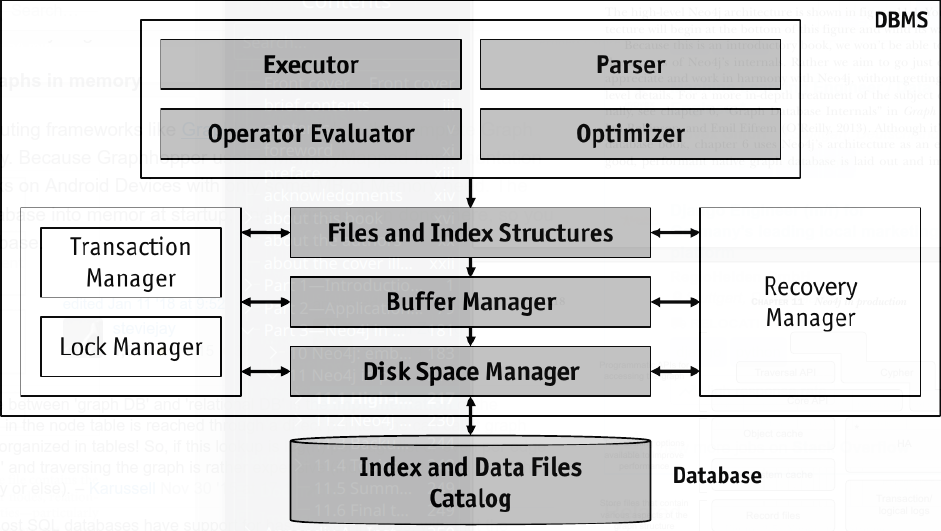
\includegraphics[keepaspectratio,width=0.7\textwidth]{img/00_intro/RDBMS.png}
        \end{center}
        \caption{The typical structure of a relational database management system.} %TODO citation
        \end{figure}

        Here The disk space manager, sometimes also called storage manager, handles de-/allocations, reads \& writes and provides the concept of a page: A disk block brought into memory. 
        For that it needs to keep track of free blocks in the allocated file. Optimally both a disk block and a page are of the same size. 
        One crucial task of a disk space manager is to store sequences of pages into continuous memory blocks in order to optimize data locality.
        Data locality has the upside, that one needs only one I/O operation to load multiple pages.
        To summarize the two most important objectives of a storage manager are to provide a locality-preserving mapping from pages to blocks based upon the information in the DBMS and to abstract physical storage to pages, taking care of allocation and access.
        
        A buffer manager is used to mediate between external storage and main memory. It maintains a designated pre-allocated area of main memory --- called the buffer pool --- to load, cache and evict pages into or from main memory.
        It's objective is to minimize the number of disk reads to be executed by caching, pre-fetching and the usage of suitable replacement policies. 
        It also needs to take care of allocating a certain fraction of pages to each transaction.

        \begin{figure}[htp]\label{dbms_memory}
            \begin{center}
            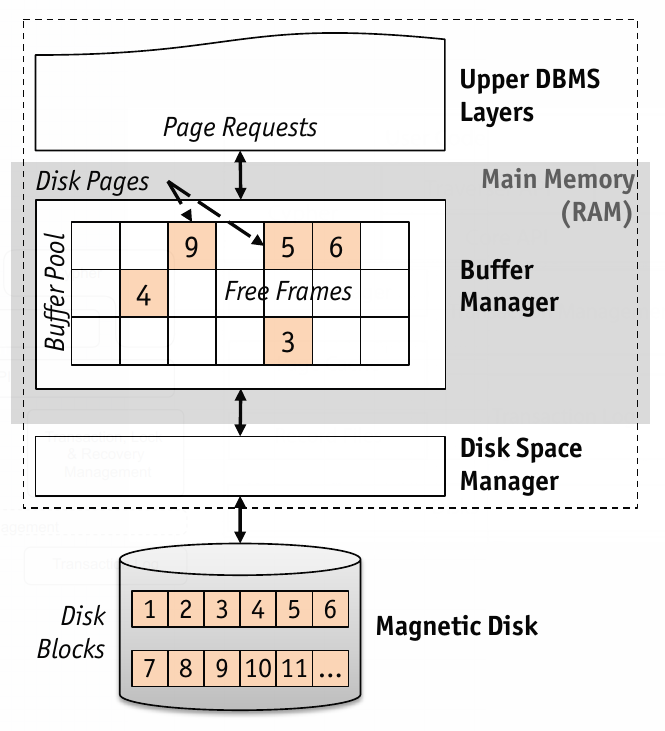
\includegraphics[keepaspectratio,height=0.4\textheight,width=0.5\textwidth]{img/00_intro/RDBMS_memory_view.png}
            \end{center}
            \caption{A visualization of the interaction of a database with memory.} %TODO citation
        \end{figure}

        The final memory and storage model relevant component of the  of a database management system is the file layout and possible index structures. 
        In order to store data a DBMS may either store one single or multiple files to maintain records. 

        A file may consist of a set of pages containing a set of slots. A slot stores one record with each record containing a set of fields. Further the database needs to keep track of free space in the file: A linked list or a directory must record free pages and some structure needs to keep track of the free slots either globally or per page. 
        Records may be of fixed or of variable size, depending on the types of their fields. 
        Records can be layout in row or column major order.
        That is one can store sequences of tuples or sequences of fields.
        The former is beneficial if a lot of update, insert or delete operations are committed to the database, while the latter optimizes the performance when scans and aggregations are the most typical queries to the system.
        Another option is to store the structure of the records along with pointers to the values of their fields in one files and the actual values in one or multiple separate files. 
        Also distinct types of tables can be stored in different files. 
        For example entities and relations can be stored in different files with references to each other, thus enabling the layout of these two to be specialized to their structure and usage in queries.

        Files may either organize their records in random order (heap file), sorted or using a hash function on one or more fields. 
        All of these approaches have upsides and downsides when it comes to scans, searches, insertions, deletions and updates. 

        To mitigate the effect that result from selecting one file organization or another, the concept of indexes have been introduced. 
        Indexes are auxiliary structures to speed up certain operations that depend on one field. 
        Indexes may be clustered or unclustered. 
        An index over field $F$ is called clustered if the underlying data file is sorted according to the values of $F$. 
        An unclustered index over field $G$ is one where the file is not sorted according to $G$. 
        In a similar way indexes can be sparse or dense. 
        A sparse index has less index entries than records, mostly one index entry per file. 
        This can of course only be done for clustered indexes as the sorting of the data file keeps the elements between index keys in order. 
        An index is dense if there is a one to one correspondence between records and index entries. 
        There are different variants of storing index entries which have again certain implications on the compactness of the index and the underlying design decisions.

        In another view of database management systems architectures, this boils down to the design decisions one has to make when implementing the storage layer and the access layer as shown in figure~\ref{dbms_arch_layers}.

        \begin{figure}[htp]\label{dbms_arch_layers}
        \begin{center}
        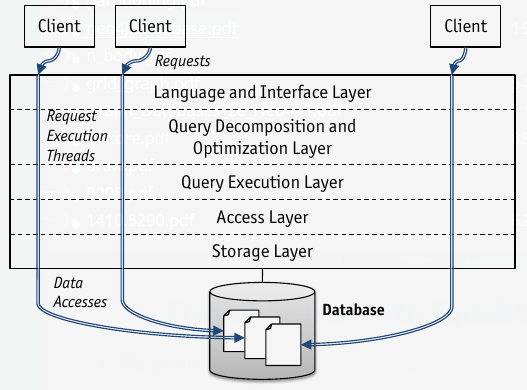
\includegraphics[keepaspectratio,width=0.6\textwidth]{img/00_intro/layered_RDBMS.png}
        \end{center}
        \caption{The architecture of a database management system from another point of view.} %TODO citation
        \end{figure}

        Here the storage layer is in close correspondence to the disk space manager in combination with the buffer manager, while the files and index structures provide the access layer.

        All these considerations make choosing different file splits, layouts, orderings, addressing schemes, management structures, de-/allocation schemes and indexes a complex set of dependent choices. 
        These depend mainly on the structure of the data to be stored and the queries to be run.


    \subsection{The Property Graph Model}\label{\positionnumber}
        The property graph model is a widely adopted data model to represent graphs in databases.
        It is not only able to represent the structure of directed or undirected, weighted or unweighted, but also of typed graphs carrying additional information.
    
        A \textbf{Property Graph} is a 9-Tuple $G = (V, E, \lambda, P, T, L, f_P, f_T, f_L)$ with 
        \begin{itemize}
            \item $V$ the set of vertices.
            \item $E$ the set of edges.
            \item $\lambda: (V \times V) \rightarrow E$ a function assigning a pair of nodes to an edge.
            \item $L$ a set of strings used as labels.
            \item $P$ a set of key-value pairs called properties.
            \item $T$ a set of strings used as relationship types.
            \item $f_P: V \cup E \rightarrow 2^P$ a function that assigns a set of properties to a node or relationship.
            \item $f_T: E \rightarrow T$ a function that assigns a type to  a relationship.
            \item  $f_L: V \rightarrow 2^L$ a function that assigns a node a set of labels.
        \end{itemize} 
        \smallskip
        The property graph model reflects a directed, node-labeled and relationship-typed multigraph $G$, where each node and relationship can hold a set of key-value pairs~\cite{angles2018property}. \\
        In a graph the edges are normally defined as $E \subseteq (V \times V)$, but in the property graph model edges have sets of properties and a type, which makes them records on their own. 
        This means they either need to be addressed explicitly or one needs to store all information, including the properties, consecutively. 
        The latter approach has the downside, that when the type or a property contain a variable length string, the relationships have to be variable lenght records. 
        This would cause the lookup of a relationship's property to be not only indirected via a node index, but also requires an additional mechanism to be able to tell the beginning and length of the record. \\
        An illustration of this model is shown in \fullref{fig:propertygraph}\fig{img/property_graph_elements.jpg}{propertygraph}{A visualization of the property graph model}{1}.
        Neo4j is a graph database employing the property graph model~\cite{neo4j_book}, which is used in the evaluation part of this thesis.
    
    \subsection{Example: Neo4J}\label{\positionnumber}
        When restricting to graph structures where nodes and relationships are allowed to have properties and labels and types respectively, this allows one to narrow down some of the design decisions.
        In particular the example of a popular graph native database --- Neo4J --- is what we discuss in this subsection.

        To get an overview of the architecture let us consider figure~\ref{N4J_HLA_Emil}. 

        \begin{figure}[htp]\label{N4J_HLA_Emil}
        \begin{center}
        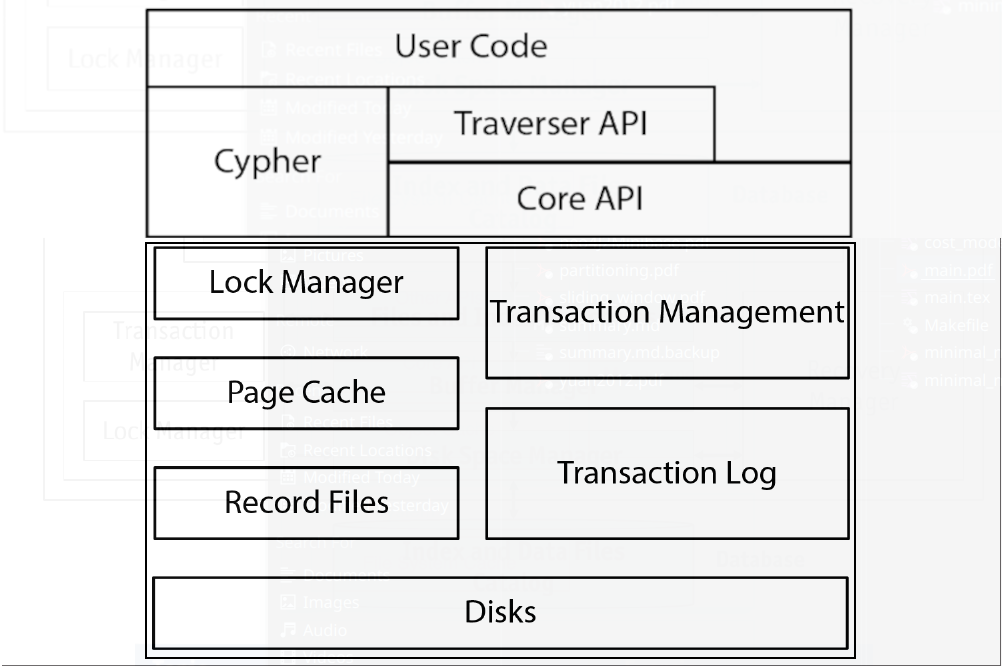
\includegraphics[keepaspectratio,width=0.6\textwidth]{img/00_intro/N4J_HLA_Emil.png}
        \end{center}
        \caption{The high level architecture of Neo4J according to Emil Efrim, the co-founder of Neo technologies.} %TODO citation
        \end{figure}

        Here we can see that the previous schema is not exactly straight forward to apply, mainly due to a lack of concise documentation.
        The diagram was taken from the only publication that elaborates on the internals of Neo4J aside from the code of course.
        
        \begin{figure}[htp]\label{N4J_Storage}
        \begin{center}
        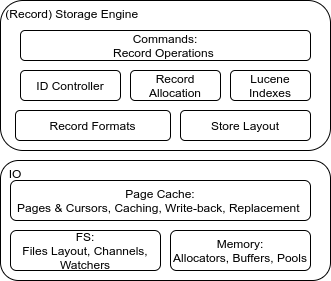
\includegraphics[keepaspectratio,width=0.5\textwidth,height=0.3\textheight]{img/00_intro/N4J_Storage.png}
        \end{center}
        \caption{A visualization of the broad the storage and memory organization of Neo4J.} %TODO citation
        \end{figure}
        
        Here The storage manager makes mostly use of the Java NIO package with some additional usage of operating system native calls to allocate memory for the page cache and network buffers. 
        A more detailed view on the high level architecture of the disk space and buffer manager and the files and index structures was deduced by the author from the source code and the non-public JavaDocs.
        This is shown in figure~\ref{N4J_Storage}.
        
      \begin{figure}[htp]\label{N4J_memory_view}
        \begin{center}
        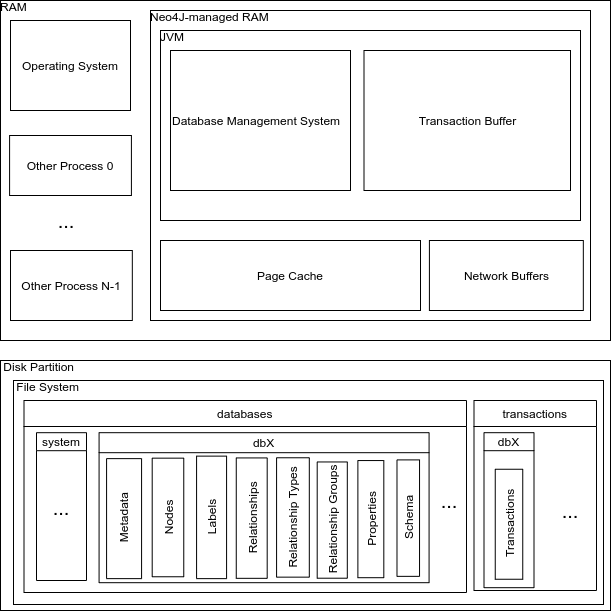
\includegraphics[keepaspectratio,width=0.6\textwidth]{img/00_intro/N4J_memory_view.png}
        \end{center}
        \caption{A sketch of how Neo4J occupies memory.} %TODO citation
        \end{figure}
        
        The overall memory and storage state of a Neo4J instance and its environment may thus be visualized like this figure~\ref{N4J_memory_view}.

        \subsubsection{IO \& File Layout}\label{files_sec}
        The files that Neo4J uses to store data are categorizable into 5 classes based upon the records they contain:
        \begin{itemize}
            \item Node-related files: These files start with the prefixes \mintinline{bash}{neostore.nodestore*} and \mintinline{bash}{neostore.label*}. 
                The contents of these files contain the node structure and labels. 
            \item Relationship-related files: The prefix \mintinline{bash}{neostore.relationship*} is used for all files containing records related to the graph's relationship structure, types and possibly groups.
            \item Property-related files: Containing the properties of both nodes and relationship, this is the part that is least structured and rather unspecialized with respect to graphs.
            \item Schema: Files starting with \mintinline{bash}{neostore.schemastore*} contain information about the schema of the graph or rather the schematic information on the node, relationship and property labels, types and constraints.
            \item Metadata: Files only starting with \mintinline{bash}{neostore} and none of the above prefixes contain meta information about the graph.
            \item Finally, a lock file.
        \end{itemize}
        
        \begin{figure}[htp]\label{files}
            \begin{center}
                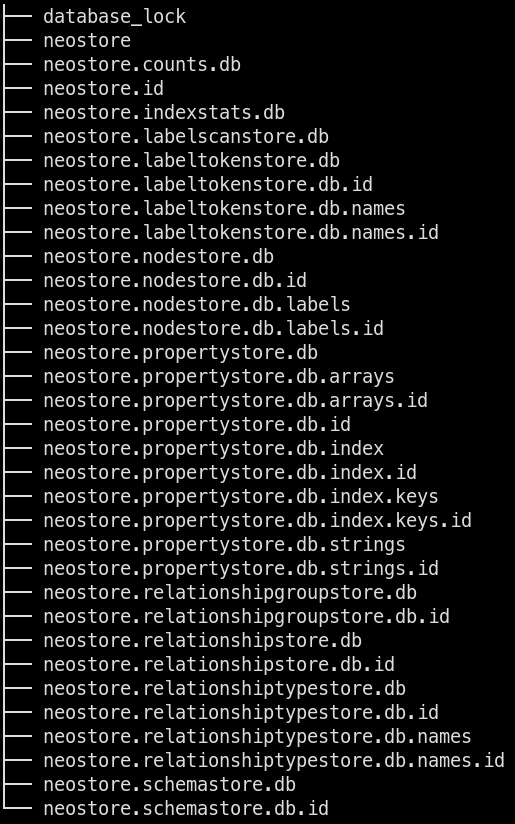
\includegraphics[keepaspectratio,height=0.4\textheight,width=0.5\textwidth]{img/03_record/files.png}
            \end{center}
            \caption{A visualization of the files layout of Neo4j.} %TODO citation
        \end{figure}

        Most importantly the files ending with \mintinline{bash}{.db} contain all fixed size records representing the structure of the graph and small amounts of data.
        Files ending with \mintinline{bash}{.id} are used for record allocation and contain unused IDs. 
        Files having one of the suffixes \mintinline{bash}{names}, \mintinline{bash}{arrays} and \mintinline{bash}{strings} are so called dynamic stores and contain dynamic sized records. 
        A dynamic store is always started with a header block containing extra information and the offset to the first block in the store files. 
        Files ending with \mintinline{bash}{.index} contain indexes either generated by Neo4J (e.g.\ the keys of properties are referenced like this to avoid storing key names multiple times) or by the Apache Lucene indexing library.
        
        \subsubsection{Record Structures}
            \paragraph{Address Translation}
                Neo4j defines the following constants as the size of the addresses used.
                \begin{figure}[htp]\label{addrsize}
                    \adjustbox{varwidth=\textwidth, scale=0.9}{%
                        \inputminted{Java}{code/MaxIdLength.java}
                    }
                \end{figure}
                These are represented by the datatype \mintinline{java}{long} when loaded into main memory. 
                On disk these values are stored as 32-bit \mintinline{java}{Integer}s with additional modifiers, that is the highest bits that do not fit into an int are stored to fields with additional space.
                
                For example the in-use bit consumes one byte of memory and the additional 7 bytes are used to stroe the highest bits that do not fit into an integer of another field.
                
                Finally the base and the modifer are aggregated into a long by shifting both appropriately, casting them to longs and applying the logical or \mintinline{java}{|} operation.
                
                Thus when refering to high bits and ID below, high bits do always mean the remainer of the bits that did not fit into the field that is said to be holding the ID\@.
                The latter is actually only holding the lowest 32 bits of an ID/address. The \textit{actual ID} is always high bits and ID field, shifted appropriately and connected using the logical or operator.
                
            \paragraph{Nodes}
                The record format of nodes consist of a 15 byte structure.
                The IDs of nodes are stored implicitly as their address.
                If a node has ID 100 we know that its record starts at offset $15 \text{ Bytes} \cdot 100 = 1500$ from the beginning of the file.
                The struct of a record looks like this:
                \begin{enumerate}
                    \item Byte 1: The first byte contains one bit for the in-use flag. 
                        The additional 7 bits are used to store the 3 highest bits of the relationship ID and the 4 highest bits of a property ID\@.
                    \item Bytes 2 --- 5: The next 4 Bytes represent the ID of the first relationship in the linked list containing the relationships of the considered node.
                    \item Bytes 6 --- 9: Again 4 bytes encode the ID to the first property of the node.
                    \item Bytes 10 --- 14: This 5 byte section points to the labels of this node.
                    \item Byte 15: The last byte stores if the node is dense, i.e.\ one node has an aweful lot of relationships and is treated a bit differently.
                        That is a relationships are stored by type and direction for this node into groups, see~\ref{rel_group}.
                \end{enumerate}
            
                \begin{figure}[htp]\label{node_record}
                    \begin{center}
                        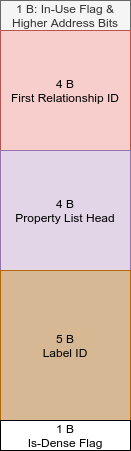
\includegraphics[keepaspectratio,height=0.4\textheight,width=0.5\textwidth]{img/03_record/node/node_record.png}
                    \end{center}
                    \caption{A visualization of the record structure of a node.} %TODO citation
                \end{figure}
                
                To summarize: The records on disk are stored as in the enumeration above. 
                In the database all IDs get mapped to longs and their respective space is larger than the space representable by 35 bit --- what is perfectly fine.
            
                \begin{figure}[htp]\label{node_first_byte}
                    \begin{center}
                        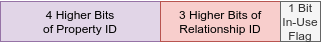
\includegraphics[keepaspectratio,height=0.4\textheight,width=0.5\textwidth]{img/03_record/node/node_first_byte.png}
                    \end{center}
                    \caption{A visualization of the information stored in the first byte of a node record.} %TODO citation
                \end{figure}
            
                On disk 4 byte integers are used to store the 32 lowest bits of the respective addresses and the higher bits are stored in the first byte that also carries the in-use bit.
            
            \paragraph{Node Labels}
                Each node label record consists of an in use bit and a name ID, which in turn points to an entry in a seperate file storing label names as dynamic records (see~\ref{dynamic}), storing the label names.
                This is done in order to assure that the records are of fixed length.
                \begin{enumerate}
                    \item Byte 1: In-use flag
                    \item Bytes 2 --- 5: Pointer to the label string entry
                \end{enumerate}
                
                \begin{figure}[htp]\label{label_record}
                    \begin{center}
                        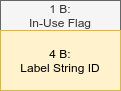
\includegraphics[keepaspectratio,height=0.2\textheight,width=0.2\textwidth]{img/03_record/node/label_record.png}
                    \end{center}
                    \caption{A visualization of the structure of a label record.} %TODO citation
                \end{figure}
                
                
            
            \paragraph{Relationships}
                \begin{figure}[htp]\label{rel_record}
                    \begin{center}
                        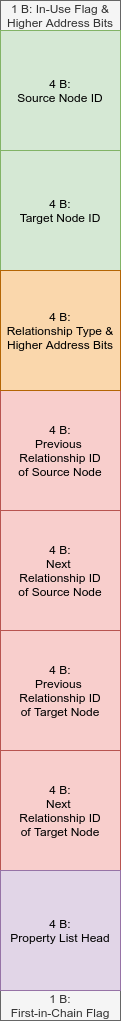
\includegraphics[keepaspectratio,height=0.9\textheight,width=0.5\textwidth]{img/03_record/relationship/relationship_record.png}
                    \end{center}
                    \caption{A visualization of the record structure of a relationship in Neo4J.} %TODO citation
                \end{figure}
                
                Relationship records are stored with implicit IDs too. 
                Their fixed size records contain 34 bytes.
                Besides an in-use flag and the node IDs that are connected, and the relationship type, the record also contains two doubly linked list: One for the relationships of the first node and one for the relationship of the second node.
                Finally a link to the head of the properties linked list of this relationship and a marker if this relationship is the first element in the relationships linked list of one of the nodes.
                \newpage
                
                \begin{enumerate}
                    \item Byte 1: In-use bit, first node high order bits (3 bits), first property high order bits (4 bits)
                    \item Bytes 2 --- 5: first node ID 
                    \item Bytes 6 --- 9: second node ID 
                    \item Bytes 10 --- 13: relationship type (16 bit), second node high order bits (3 bits), relationship previous and next ID higher bits for first and second node ($4 \cdot 3 = 12$ bits), one unused bit.
                    \item Bytes 14 --- 17: previous relationship ID for first node
                    \item Bytes 18 --- 21: next relationship ID for first node
                    \item Bytes 22 --- 25: previous relationship ID for second node
                    \item Bytes 26 --- 29: next relationship ID for second node
                    \item Bytes 30 --- 33: link to the first property of the relationship
                    \item Bytes 34: A marker if this relation is the first element in the relationship linked list of one of the nodes stored in the lowest two bits of the byte. 
                        The other 6 bits are unused.
                \end{enumerate}


                \begin{figure}[htp]\label{rel_first_byte}
                    \begin{center}
                        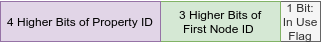
\includegraphics[keepaspectratio,width=\textwidth]{img/03_record/relationship/relationship_first_byte.png}
                    \end{center}
                    \caption{A visualization of how information is stored in the first byte of a relationship record.} %TODO citation
                \end{figure}

                \begin{figure}[htp]\label{rel_type_bytes}
                    \begin{center}
                        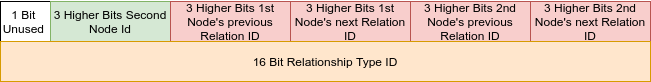
\includegraphics[keepaspectratio,width=\textwidth]{img/03_record/relationship/relationship_type_bytes.png}
                    \end{center}
                    \caption{The structure of the bytes that are used to store the type of a relationship and high bits of a node and a relationship IDs.} %TODO citation
                \end{figure}
            

            \paragraph{Relationship Types}
                Similarly to the node labels, the relationship type records posses an in-use flag and a type ID that points to a record in a file containing strings in the dynamic record format.
                \begin{enumerate}
                    \item Byte 1: In-use flag
                    \item Bytes 2 --- 5: Pointer to the type string entry
                \end{enumerate}
            
                \begin{figure}[htp]\label{rel_type_record}
                    \begin{center}
                        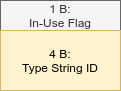
\includegraphics[keepaspectratio,height=0.2\textheight,width=0.2\textwidth]{img/03_record/relationship/rel_type_record.png}
                    \end{center}
                    \caption{A visualization of the record structure of a relationship type.} %TODO citation
                \end{figure}
                
           
           All further record structures like properties, arrays and strings are omitted for the sake of succintness.
        
        \subsubsection{Caching \& Indexes} 
        
        \subsubsection{Queries \& Transactions}
            
            
\section{Locality}\label{\positionnumber}
    
    \subsection{Metrics}
    
    
\section{Problem Definition}\label{\positionnumber}



\chapter{Problem Definition}\label{\positionnumber}
\section{Locality}\label{\positionnumber}
    The memory hierarchy was introduced in \ref{db-arch} and \ref{mem-hier}. 
    In summary it tries to unify the strengths of fast, low capacity memory --- caches (SRAM) ---, with slower but larger memory --- main memory (DRAM), with orders of magnitude slower but orders of magnitude larger memory --- disks (HDD) and more recently flash memory (SSD, SD-Cards).
    But how can this actually work? 
    Given that only a tiny fraction of fast memory is available to hold the necessarry parts, while additional loads of data are transfered in time --- ``desirably fast enough''.
    
    The key principle for the memory hierarchy to work is what is called \textit{locality of reference} in the literature~\autocite{jacob2010memory, tanenbaum2015modern}. 
    This principle expresses, that most programs do not access their address space uniformly or randomly, but rather tend to access small subsets of all addresses in certain time intervals, depending on the program state.
    Locality comes in two flavors: 
    
    \begin{itemize}
     \item \textit{Temporal locality} refers to the number of other references between two accesses of the same memory location. 
     \item \textit{Spatial locality} refers to the number of accesses and the radius of the neighbourhood that is accessed in a number of steps.
    \end{itemize}
    
    If the same location is accessed multiple times in a short amount of time, the temporal locality is high.
    Thus temporal locality can be measured using reference frequencies.
    From a bayesian point of view, one can say that temporal locality is the probability of an object being rereferenced after the first usage~\autocite{gupta2013locality}. 
    \[ P (X_{t + \Delta} = A | X_t = A) \]
    $X_t$ is the reference at time step $t$, $A$ is an address and $\Delta$ is a parameter, which depends not only on the system specifications (like the CPU and memory clock), but also on the program and the scale of interest.
    
    If a small range of addresses is accessed very often then spatial locality is high.
    If the range is limited to one address, then spatial locality is equivalent to temporal locality. Thus temporal locality is a special case of temporal locality~\autocite{gupta2013locality}.
    With $\varepsilon$ a radius we can characterize spatial locality by:
    \[ P(X_{t + \Delta} = A \pm \varepsilon | X_t = A) \]
    Spatial locality is thus a function of time $\Delta$ and neighbourhood range $\varepsilon$. 
    
    In order to leverage these concepts, several components profile the memory usage.
    In the memory hierarchy, all on and off chip caches (i.e. SRAM) are handled by hardware~\autocite{jacob2010memory}.
    
    At the level of main memory (DRAM), the operating system manages what is fetched, buffered and evicted from disk to main memory. 
    The optimal buffering strategy is to load what is needed before its usage and evict the objects whos usage is furthest in the future~\autocite{tanenbaum2015modern}. 
    
    When it comes to eviction the best approximation to the optimal strategy is the least recently used algorithm. 
    It aims to keep things in memory, that have the highest chance to exhibit temporal locality.
    That is, the things in memory, that have not been referenced for the longest time, have a lower chance to be temporally local in the future~\autocite{silberschatz2006operating}.
    Put differently \textit{caches and buffers exploit temporal locality}.
    
    As this information is not available in general, objects are loaded when they are referenced, often with additional addresses which are hoped to be needed, too --- this is called prefetch or predicitve fetching~\autocite{stallings2012operating, jacob2010memory}. 
    Prefetch tries to exploit spatial locality. There are several components that try to exploit this:
    \begin{itemize}
     \item Compiler generated prefetches: 
     The compiler knows what addresses the program accesses in which sequence and tries to minimize the time that is spent waiting for IO. 
     This is called instruction scheduling~\autocite{aho1986compilers}. 
     Other compiler generated heuristics are applied e.g. in domain specific compilers, like in the TVM compiler for neural networks~\autocite{chen2018tvm}.
     
     \item The operating system may use specialized data structures and algorithms to estimate, if prefetching should be done, based on the previous accesses. 
     An example is the ``spatial look-ahead'' algorithm by Baier and Sager~\autocite{jacob2010memory, baier1976dynamic}, but there exist many more e.g. \autocite{joseph1999prefetching, griffioen1994reducing, kroeger1997exploring, cooksey2002stateless}. 
     Most of these methods are capable to find correlations between addresses and their neighbourhood, file accesses and pointed-to objects.
     
     \item A special role in the context of prefetches and spatial locality take databases. 
     As these are not only able to predict content-based correlations, e.g. by knowing what table is queried in the case of relational databases, but also can augment data by using auxiliary data structures like indices. 
     The most remarkable capability in this context is to be able to reorganize data, based upon how it is queried.
     Relational databases store data in tables and often sort these tables based upon either a certain field (like the primary key) or a set of fields. 
     This in combination with being able to analyze the query before executing it allows reordering the memory accesses, such that as many accesses as possible are sequential~\autocite{ramakrishnan2000database, silberschatz1997database}.
    \end{itemize}
    
    Spatial locality depends on how data is ordered:
    If semantically closely coupled data is spread out as wide as possible, the program or file of interest will harldy exhibit locality. 
    As an example consider a program with $n$ instructions, with logical addresses from $0, \dots, n-1$. 
    An inversion is a change of position of two lines $l_1, l_2$, such that the line that gets executed earlier $l_1$ has a higher address than one that gets executed later $l_2$.
    Such a program can maximally have $\frac{n (n-1)}{2}$ inversions. 
    If it has that many inversion, the program is layed out in the opposite direction and the spatial locality would be similar to the original program.
    Thus lets assume only every second instruction is misplaced. 
    In effect, to execute the program two pages must always remain in memory instead of one and the radius of the neighbourhood doubles.
    
    In short: 
    The layout of the data or records in the address space --- on file or in memory --- is crucial to the concept of spatial locality. 
    Achieving optimal temporal locality is a matter of grouping and ordering data such that what is referenced together is in a neighbourhood in terms of addressing.
    
          
\section{Problem Definition}\label{\positionnumber}
    In order to optimize spatial locality for traversal-based queries, the graph needs to be grouped and ordered.
    Ultimately disk storage is block-based and disk access is page-based. 
    That is the vertices and edges must be grouped into blocks.
    
    \paragraph{Assumptions:}
    In the remainder of this thesis we are assuming that the graph is represented in the property graph model~\ref{prop-graph-model} and uses incidence lists~\ref{inci} as the storage schema. 
    We are not taking properties, labels and relationship types into account.
    We are focusing on spatial locality here, that is the page replacement algorithm is fixed but arbitrary.
    Finally in the remainder of the thesis when talking about traversal-based queries, we mean all queries described in \ref{queries}, but the random walk.
    
    \paragraph{Problem Definition:} Given a graph $G$, logical block size $b$, page size $p$. \\
    Desired is 
    \begin{enumerate}
     \item A partition of $G$ into blocks of vertex records $V_i$ and $E_i$ relationship records, 
     \item orderings or permutations $\pi_v, \pi_e$ of the blocks of vertex and edge records $V_i, E_i$,
     \item a reordering of the incidence list pointers
    \end{enumerate}
    such that spatial locality is as high as possible for traversal-based queries.
    
    As partitioning a graph optimally~\autocite{andreev2006balanced}, as well as finding an optimal linear arrangement~\autocite{garey1974some} are both NP-complete problems~\autocite{lewis1983computers}, we use the formulation ``as high as possible'' instead of optimal or maximal.
    
    In order to measure the spatial locality we introduce two measures that are used in the evaluation chapter:
    \begin{enumerate}
     \item Number of block accesses.
     \item Number of non-consecutive block accesses.
    \end{enumerate}
    The first measure is to take the neighbourhood within a block into account: If vertices and edges that are accessed together are stored in the same block, this measure should be as small as possible.
    The second measure takes the order of the blocks into account: 
    If vertices and edges that are connected or ``close'' to each other are stored in adjacent blocks, they can be loaded with one sequential read.
    But the second measure also takes into account how the traversal is executed in terms of pointer chasing with respect to the incidence list.
    
\section{Example: Vertex, Edge and Incidence List Order}
  Why are these three criteria neccessary? Why are there only two measurements for three criteria? \\
  This is what shall be explained in an example.
  Something that is of importance for the traversal --- but not as straight forward to see as node and edge grouping and order --- is the order of the pointers in the incidence list, as we are going to see.
  
  \begin{figure}[htp]
    \begin{center}
        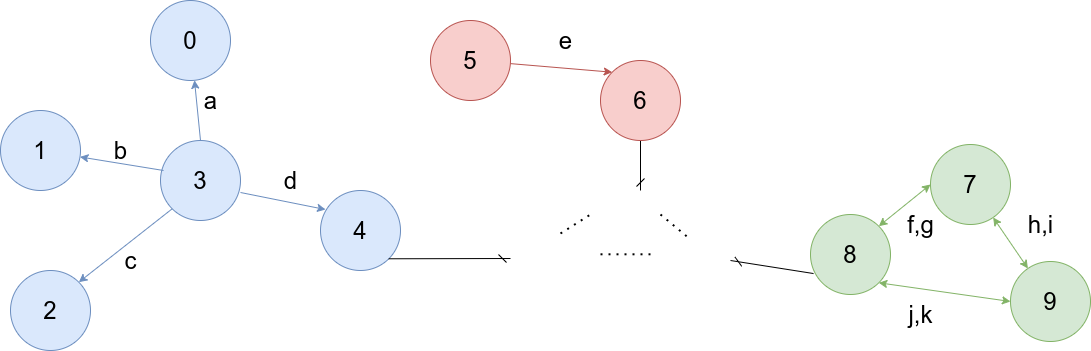
\includegraphics[keepaspectratio,height=0.3\textheight,width=\textwidth]{img/04-problem_def/example_graph.png}
    \end{center}
    \caption{Parts of a graph that is used in subsequent examples. Cut through edges mean edges to any non-visualized component of the graph. The dotted lines indicate, that other nodes and edges are between the three shown components.}
    \label{ex-gr}
  \end{figure}
  
  The graph used in the below example looks as shown in \ref{ex-gr}.
  We use a storage schema that is motivated by the one of Neo4J, that is nodes and relationships are stored in separated files, the incidence list is stored in the records of the edges and the nodes conatain a pointer to the head relationship of their incidence list each. Further we assume that we can only read sequentially, if the blocks are directly adjacent.
  As this is a rather small example for the sake of succintness, things are just shown on a conceptual level. 
  We make the assumption that 3 nodes or 2 relationships fit onto a disk block. 
  Realistically 8 to 16 nodes and 5 to 8 relationships fit on a 512 byte disk block. 
  An average graph in the stanford network analysis platform graph dataset collection has thousands of nodes and edges. 
  Taking the californian road network graph as an example, the whole graph would take 
  \[ 1 965 206 \text{ nodes} \cdot 35 \text{ bytes per node} \cdot 512^{-1} \text{ bytes per block} = 134 341\text{ blocks}\] 
  to store all nodes and 
  \[2 766 607 \text{ relationships} \cdot 72 \text{ bytes per relationship} \cdot 512^{-1} \text{ bytes per block} = 389055\text{ blocks}\] 
  blocks to store the relationships in Neo4J.
  To summarize, the principles shown below scale with the graph size and for realistic assumptions, these conditions emerge.

  First consider the split of vertices and edges into blocks in the upper table in \ref{blocks}. 
  None of the vertices in the blocks are neighbouring to each other.
  Thus when traversing the graph, each step requires to load a block.
  The same is true for the edges: 
  None of the edges in the same block are connected to the same vertex. 
  Each edge causes a page fault and a load of another block(s).
  This may happen in current state of the art graph databases like Neo4J. 
  The placment into blocks is currently by insertion order, thus depends on the ordering of the input dataset. 
  On the other handside in the lower table in \ref{blocks}, the vertices are grouped into blocks according to their neighbourhood and the edges are grouped by the vertices they are connected to.

  
     \begin{table}[htp]
     \centering
    \begin{tabular}[c]{|l|c|c|c|c|c|c|} \hline
    &&&&&&\\[-1em]
     node.db & \colorbox{blue!30}{0}, \colorbox{red!30}{5}, \colorbox{green!30}{7} & \colorbox{blue!30}{1}, \colorbox{blue!30}{4}, \colorbox{green!30}{9} & \colorbox{blue!30}{2}, \colorbox{red!30}{6}, \colorbox{green!30}{8} & \colorbox{blue!30}{3} &  & \\ \hline
     &&&&&&\\[-1em]
     edge.db & \colorbox{blue!30}{a}, \colorbox{green!30}{f} & \colorbox{blue!30}{b}, \colorbox{green!30}{g} & \colorbox{blue!30}{c}, \colorbox{green!30}{h} & \colorbox{blue!30}{d}, \colorbox{green!30}{i} & \colorbox{red!30}{e}, \colorbox{green!30}{j} & \colorbox{green!30}{k} \\  \hline
    \end{tabular}
    \vspace{0.5cm}
    
    \begin{tabular}{|l | c | c | c | c | c | c|} \hline
    &&&&&&\\[-1em]
     node.db & \colorbox{green!30}{7},\colorbox{green!30}{8}, \colorbox{green!30}{9} & \colorbox{blue!30}{0}, \colorbox{blue!30}{1}, \colorbox{blue!30}{3} & \colorbox{red!30}{6} & \colorbox{blue!30}{4}, \colorbox{blue!30}{2}, \colorbox{red!30}{5},  &  & \\ \hline
     &&&&&&\\[-1em]
     edge.db &  \colorbox{green!30}{f}, \colorbox{green!30}{h} & \colorbox{green!30}{g}, \colorbox{green!30}{k} & \colorbox{green!30}{i}, \colorbox{green!30}{j} & \colorbox{blue!30}{a}, \colorbox{blue!30}{b} & \colorbox{red!30}{e} & \colorbox{blue!30}{c}, \colorbox{blue!30}{d} \\ \hline
    \end{tabular}
  \caption{An example of suboptimal and improved record placement into blocks. 
  The block size is assumed to be only 3 vertex records and 2 node records respectively. 
  For larger block size, the same principle applies.}
   \label{blocks}
   \end{table}
    
  Next \ref{order} shows two different orderings of the blocks, this time with a focus on the edges only. 
  In the upper table, an edge is stored in the neighbourhood of its source node, but appart from its target node.
  Thus two single reads are required to go from one vertex over an edge to another vertex and retreive it's incident edges. 
  In the lower table, the blocks are adjacent and one sequential read  is enough to go from source to target and fetch the target't incidence list.
  
     \begin{table}[htp]
          \centering
    \begin{tabular}{|l | c | c | c | c | c | c|} \hline
    &&&&&&\\[-1em]
     edge.db &  \colorbox{green!30}{f}, \colorbox{green!30}{h}   & \colorbox{blue!30}{a}, \colorbox{blue!30}{b} & \colorbox{green!30}{i}, \colorbox{green!30}{j} & \colorbox{red!30}{e} & \colorbox{blue!30}{c}, \colorbox{blue!30}{d} & \colorbox{green!30}{g}, \colorbox{green!30}{k} \\ \hline
    \end{tabular}
    \vspace{0.5cm}
    
    \begin{tabular}{|l | c | c | c | c | c | c|}\hline
    &&&&&&\\[-1em]
     edge.db &  \colorbox{green!30}{f}, \colorbox{green!30}{h} & \colorbox{green!30}{g}, \colorbox{green!30}{k} & \colorbox{green!30}{i}, \colorbox{green!30}{j} & \colorbox{blue!30}{a}, \colorbox{blue!30}{b} & \colorbox{blue!30}{c}, \colorbox{blue!30}{d} & \colorbox{red!30}{e} \\ \hline
    \end{tabular}
      \caption{Suboptimal and improved block order.}
    \label{order}
       \end{table}
  
  Finally: Consider the visualization of the incidence list of the node 3, given the page placement in the upper part of \ref{blocks} in \ref{inc-ord}. 
  Theoretically the only difference is the order in which the list points to the relationships. 
  In terms of traversed blocks, we need to do four single reads when using the order given in the upper table. 
  If we rearrange the pointers according to the lower table, the list may be loaded sequentially with one read operation instead of four single reads. 
  This phenomenon may also appear when the blocks are formed and ordered in an improved way, but only when scaling up to a graph with larger neighbourhoods.
  Given that an edge can be placed either near the other edges of the source or the target node, the impact when jumping back and forth will grow along with the gaps between blocks in which the edges are stored.
  Finally if the blocks are cached, this induces a higher load on the buffer manager, as more pages need to reside in memory at the same time and as they are frequently rereferenced instead of being read once and evicted then.
  The higher the degree --- i.e. the length of the incidence list --- of the node, the more severe the effect.
  % TODO validate!

\begin{table}[htp]
          \centering
    \begin{tabular}{|l | c | c | c | c |}\hline
     incidence list of node 3 &  c & a & d & b\\ \hline
    \end{tabular}
    \vspace{0.5cm}
    
    \begin{tabular}{|l | c | c | c | c |}\hline
     incidence list for node 3 &  a & b & c & d\\ \hline
    \end{tabular}
      \caption{Suboptimal and improved incidence list order.}
    \label{inc-ord}
       \end{table}

\chapter{Related Work}\label{\positionnumber}
\section{G-Store: Multilevel Partitioning}\label{\positionnumber}
    G-Store is a disk-based storage manager for graph data implemented and published by Steinhaus et al.~\autocite{steinhaus2010g}. 
    To the best of the authors knowledge, this is the first structured approach to improve locality in graph databases by altering the placement of records into blocks.
    More specifically, in order to maximize performance, they try to place adjacent nodes close to each other, such that they can be read sequentially. 
    The rearrangement of the records is done when importing a new data set and is static after insertion.
    G-Store uses adjacency lists as data structure and does not store these in an own file but directly next to the vertex in the very same file.
    The broad schema of the placement method developed by Steinhaus et al.~\autocite{steinhaus2010g} is derived from multilevel partitioning methods, initially published first by Hendrickson and Leland~\autocite{hendrickson1995multi} and a bit later implemented in the seminal METS framework by Karypis and Kumar~\autocite{karypis}.
    Briefly, the multilevel partitioning algorithm works in three steps: Coarsening, Turn-around and uncoarsening. 
    The coarsening phase tries to reduce the original graph to a smaller one that braodly preserves the structure of the underlying graph. 
    A more partitioning algorithm expensive algorithm can then be applied to this smaller graph to solve the actual problem approximately and fast.
    During the uncoarsening, the approximate solution is refined and the coarser graph is projected back until the original graph is mapped and restored.
    A broad overview of the method is shown in \ref{g-store}.
    
    \begin{figure}
        \begin{center}
            \includegraphics[keepaspectratio,width=0.7\textwidth]{img/05-rel_w/g-store.png}
        \end{center}
        \caption{A broad overview of the multilevel partitioning method applied by G-Store~\autocite{steinhaus2010g}.} 
        \label{g-store}
    \end{figure}

    
    In the next part of this section we are going to use the notions of a finer and a coarser graph a lot. Let therefore $G = G_0 = (V_0, E_0)$ the original graph, and $G_i = (V_i, E_i)$ the graph that was coarsened $i$ times.
    
    \subsection{Coarsening}\label{\positionnumber}
    The coarsening phase of G-Stores partitioning algorithm is what is called heavy edge matching (HEM) in Karypis formulation of the algorithm as already mentioned. 
    It works by iterating over all vertices and matching each one with the vertex that is attached to the edge carrying the heaviest weight.
    This is done until all edges are matched.
    Afterwards, all pairs of vertices form a new vertex in a new graph, the edges of each vertex pair are aggregated and their weight is summed eventually, if both nodes had an edge to the same other vertex. 
    Thus the algorithm takes $G_i$ as parameter and returns $G_{i+1}$ along with a projection $Z_{i+1}$ specifying which finer nodes maps to which coarser node.
    Further the nodes are assigned a weight that corresponds to the number of vertices that are matched in one meta-vertex.
    Coarsening proceeds in the original algorithm until a certain lower limit of vertices is reached.
    In the METIS implementation this is hard-coded to  $\max \left( 20k, 40 \log_2 k\right)$ where $k$ is a user defined parameter specifying the number of partitions.
    The algorithm used in G-Store keeps coarsening until there are no edges, i.e. only one vertex.
    It can thus be seen as a form of hierarchical agglomerative clustering with the inverse edge weight acting as a distance function.
    
    Another modification is that in contrast to METIS, not only two edges are matched at a time but possibly many and that there is an upper limit to the vertex weights. 
    This depends on the coarsening factor $c(i) = \frac{|V_i| - |V_{i+1}|}{|V_i| - |\{v \in V | N_v = \emptyset \}|}$, with $i$ the level of coarsening, where $i=0$ it the original graph.
    The counter is the number of vertices that were reduced and the denominator is the number of nodes in the larger graph minus the irreducible nodes.
    Initially the allowed vertex weight $\theta$ is the size of a block.
    If this factor $c(i) < 0.3$ then the node weight $\theta$ is doubled as long as $\theta \leq 32$.
    Otherwise the number of nodes that are allowed to be matched is incremented.
        
    \subsection{Turn-Around}\label{\positionnumber}
    In G-Store the turn-around simply assigns every vertex in the coarsest graph, whose weight is larger than the size of a block, a distinct partition number.
    The other nodes are added up until their weight reaches the size of a block and are assigned a partition number together.
    Thus the algorithm accepts a fully coarsened graph $G_i$ and returns the partition numbers for this graph $\phi_i$.

    
    \subsection{Uncoarsening}\label{\positionnumber}
    The uncoarsening phase consists of three different steps that are performed per level:
    Projection, reordering and refinement.
    Projection constructs a first mapping, reordering swaps partitions and refinement exchanges nodes between partitions.
    Each iteration of the full uncoarsening procedure takes the coarser graph $G_{i+1}$ as an argument along with its the partition numbers $\phi_{i+1}$ and the mapping $Z_{i}$ and returns the one level uncoarsened graph $G_i$, along with the respective partition numbers $\phi_i$.
    The algorithm also defines a weight threshold per level. With $\overline{c}$ the average coarsening factor
    \[ \chi_i = \lfloor \frac{\text{block size}}{(1-\overline{c})^i} \rfloor. \]
    
    Further it defines three objective functions:\\
    The first function is closesly related to the minimal linear arrangement problem~\autocite{lewis1983computers} and expresses that nodes that share an edge shall be minimally far appart from each other.
    \[ \min C_1 = \min \sum_{(u,v) \in E} |\phi(u) - \phi(v)| \]
    The second objective function aims to reduce the overall number of edges between the partitions.
    \[\min C_2 = \min \sum_{(u,v) \in E)} \begin{cases}
        1 & \phi(u) \neq \phi(v) \\
        0 & \text{ otherwise}
    \end{cases}
\]
    The last objective function penalizes the number of blocks that are linked. That is in order to reduce the number of overall linked blocks according to~\autocite{steinhaus2010g}.
    \[ \min C_3 = \min \sum_{i \leq j} 
    \begin{cases}
        1 & \phi(u) = i \wedge \phi(v) = j, \ (u,v) \in E \\
        0 & \text{ otherwise}
    \end{cases}
    \]
    
    Finally there are two functions that are similar to the first objective function that are used in the projection step called tension and modified tension:
    The tension is the weighted distance between the block of the vertices that share and edge. Let $v \in V_i$.
    \[ t(v) = \sum_{u \in N_v} w_{(u,v)} \phi_i(v) - \phi_i(u)\]
     The modified tension is just the same, but instead of using the actual graph, one uses the coarser graph $G_{i+1}$ and the projection $Z_{i}$ to estimate the tension:
     \[ t'(v) = \sum_{u \in N_v} w_{(u, v)} \phi_{i+1}(Z(v)) - \phi_{i+1}(Z(u)) \]
    
        \subsubsection*{Projection}
        This part of the algorithm constructs a first version of the finer-grained partition numbers $\phi_i$ from the coarser ones $\phi_{i + 1}$.
        The enumeration follows a dewey numbering scheme.
        That is per level one place in the partition label is added. 
        If the vertex $\phi_{i+1}(Z(v)) = 2$ and vertex $\phi_i(v) = 1$, then the overall partition label of the vertex is $2\text{.}1$. 
        
        Per partition in the coarser level graph, the algorithm either simply assigns the same partition number to all nodes $v_i \in Z(\phi{i+1,j})$ in the finer graph $G_i$ that were clustered into the recpective coarser nodes, if the overall weight of the partition in the coarser graph is smaller than the weight threshold: $w_{\phi{i+1, j}} \leq \chi_i$.
        Otherwise the modified tension is computed is computed for all nodes of the partition in the finer graph $\forall v_i \in Z(\phi{i+1,j}): t'(v_i)$.
        The minimal tension is extracted, placed to the leftmost free position in the partition and the tensions of the neighbours are updated. 
        This is done repeatedly until all nodes are placed.
        During this step, each partition is marked with a flag, that is true, when it was created from nodes in the right half of the coarser partition.
                
        \subsubsection*{Reordering}
        When swapping the above created partitions, only $C_1$ changes, but not $C_2$ or $C_3$. Using the just created flags, groups are identified which span two half coarser partitions $\phi_{i+1,j}, \phi_{i+1,j+1}$. Per group the finer partitions are swapped as long as the overall absolute tension ($C_1$) decreases by some swap.
        In effect, this is a fix-point computation.
        
        \subsubsection*{Refinement}
        Finally the refinement step tries to optimize a weighted sum of all the objective functions by moving vertices to other partitions.
        Three used-defined parameters $\alpha, \beta, \gamma$ control the weighting, another one specifies the number of iterations that shall be executed $r$.
        In each iteration, the algorithm steps over the partitions $\phi_{i,j}$ and creates a two dimensional array $A$ of dimension $|\phi_{i,j}| \times |P_{i,j}|$ with $P_{i,j} = \{ \phi_i(u) | v \in \phi_{i,j}, u \in N_n\} \setminus \phi_{i,j}$.
        Each entry is defined with $v$ the vertex that is to be moved to partition $k$:
        \[ a_{v,k} = \alpha C_1 + \beta C_2 + \gamma C_3 + \lambda \]
        Where $\lambda$ penalizes overfull blocks or rewards the filling of less filled blocks.
                
    \subsection{Finalization}
    The finalization algorithm implements a final pass over all so formed partitioning schema, that converts partitions into blocks of adequate size and balances less filled partitions.
    
\section{ICBL: Diffusion Set-based Clustering}\label{\positionnumber}
    Ya\c{c}ar and Gedik propose another method to form and order blocks~\autocite{yacsar2015scalable, yacsar2017distributed}. 
        
    They define one metric for each of the task:
    \textit{Block locality} is defined by the means of conductance and cohesiveness. 
    Conductance is defined as the ratio of edge cuts to total edges in a block:
    \[ C_d (B) = \frac{|\{ (u,v) \in E: |\{u,v\} \cap V_B| = 1\}|}{|\{ (u,v) \in E: |\{u,v\} \cap V_B| > 0\}|} \]
    Cohesiveness is the number of nodes in the same blocks that are connected by an edge divided by the number of theoretically possible edges, i.e. $|V|^2$ in a directed graph. The authors assume an undirected self-loop free graph, thus the number of possible edges is $\frac{|V| (|V| - 1)}{2}$.
    \[ C_h (B) = \frac{|\{ (u,v) \in E: u,v \in V_B \}|}{|V|^2} \]
    As conductance takes edges between blocks into account and cohesiveness meausures the edges within a block, they are complementary~\autocite{yacsar2015scalable}.
    Thus the locality of a block us defined as the geometric mean of the measures above, where the conductance is subtracted from one:
    \[ L(B) = \sqrt{C_h (B) \cdot (1 - C_d (B))} \]
    \textit{Ranking locality} is related to what we called tension before. 
    Here we do not measure it between partitions of the node but directly to the position in the order. 
    Let $v \in V$ a node and $r(v)$ a function that assigns a natural number in the range of $\{0, \dots, |V|-1\}$ to each vertex.
    \[ R (v) = \sum_{u \in N_v} r(v) - r(u) \]
    The locality of a block is then defined by one minus the normalized average distance for all vertices in the block:
    \[ R(B) = 1 - \frac{1}{(|V| - 1)} \sum_{v \in V_B} \frac{R(v)}{|N_v|} \]
    
    \begin{figure}[htp]
        \begin{center}
            \includegraphics[keepaspectratio,width=0.8\textwidth]{img/05-rel_w/icbl.png}
        \end{center}
        \caption{A broad overview of the ICBL method by Ya\c{c}ar and Gedik~\autocite{yacsar2015scalable}.} 
        \label{icbl}
    \end{figure}

    ICBL is an acronym for the single steps performed by this algorithm. 
    It is designed to be implemented and executed using the map-reduce model.
    First ICBL extracts so called diffusion sets as features.
    Then it clusters the vertices based upon these features, to split the graph into subgraphs.
    After that it hierarchically clusters the subgraphs obtained in the previous step in order to form blocks.
    Finally the just formed blocks are ranked and layed out on disk.
    A brief visualization of the method is shown in~\ref{icbl}.
    
    \subsection{Identify Diffusion Sets}\label{\positionnumber}
    The diffusion set $\mathcal{D}_v$ of a vertex $v \in V$ is a characterization of the surrounding of a vertex. 
    A surrounding means other vertices that are reachable in a certain number of steps.
    To identify the diffusion set, ICBL carries out $t$ random walks (\ref{rand-w}, \ref{random_walk}) of length $l$.
    The authors characterize a random walk using the vertices so from out definition we need to extract the multiset of vertices from the walk.
    
    For choosing the parameters $t$ and $l$ Ya\c{c}ar and Gedik propose heuristics: 
    For $t$, construct the cumulative degree distribution $f(d) \mapsto P(x \leq d)$ and chose the minimal degree value such that the derivative of the cumulative degree distribution $f'(d) = 1$. The value of the derivative was derived empirically.
    Regarding $l$ the authors make the assumotion that the network exihibits the small world phenomenon~\autocite{kleinberg2000small}.
    In a network that has that property, the probability is high that there exists a path between any two nodes $u,v \in V$ of length $\ln{|V|}$.
    In order to construct diffusion sets that are characterizing, the length of the random walk should not be too long as all nodes might be visitable then. Thus the heuristic for choosing $l$ is $1 + \lceil \frac{\ln |V|}{k} \rceil$ where $k$ is the number of clusters in the next step.
    
    \subsection{Coarse Clustering}\label{\positionnumber}
    After generating the diffusion sets, the graph is clustered using a variation of the k-Means algorithm~\autocite{lloyd1982least}. 
    It is used to partition the graph into $k$ smaller subgraphs, such that the computationally more expensive agglomerative hierarchical clustering~\autocite{hac} algorithm that is used in block formation can be executed in parallel.
    Instead of using a geometric distance function (like the manhatten or the euclidean distance between points on a plane), an alternated version of the Jaccard distance function~\autocite{jaccard1912distribution} is used. 
    The Jaccard function $J(u, v) = 1 - \frac{\mathcal{D}_u \cap \mathcal{D}_v}{\mathcal{D}_u \cup \mathcal{D}_v}$, i.e. the distance is the number of common elements divided by the set of all elements in both sets. 
    The altered distance is adjusted for multisets:  
    \[J_w (u, v) = 1 - \frac{\sum_{x \in \mathcal{D}_v \cap \mathcal{D}_u} \min (w_{\mathcal{D}_v}, w_{\mathcal{D}_u})}{\sum_{x \in \mathcal{D}_v \cup \mathcal{D}_u} \max (w_{\mathcal{D}_v}, w_{\mathcal{D}_u})} \]
    First $k$ initial centers are chosen based upon the node degree and the distance to the already chosen centers.
    Then all nodes get assigned to the closest center. 
    After that the centers are updated, by building the union of all diffusion sets and use the vertex with the highest weight as new center.
    This is done until the centers do not change further.
    In order to determine the number of clusters, the authors propose a heuristic that is based on the available memory $M$ and the size of a vertex and the average diffusion set $s = \text{sizeof}(v) + \overline{\text{sizeof}(\mathcal{D})}$: 
    \[ k = \lceil \frac{s \cdot |V|}{\sqrt{0.8 \cdot M}} \rceil \]
    
    \subsection{Block Formation}\label{\positionnumber}
    For each subgraph, agglomerative hierarchical clustering~\autocite{hac} is used to form blocks and label them for the ranking process.
    Each vertex starts in an own partition. 
    In every step the two closest partitions are merged. 
    The distance function here is the minimum of the previously defined weighted Jaccard distance of all nodes in the partition:
    \[ J_P (P_i, P_j) = \argmin_{u \in P_i, v \in P_j} J_w (\mathcal{D}_u, \mathcal{D}_v) \]
    Each partition maintains a label, that is used subsequently.
    In the beginning the node id is used as label. 
    When a potential merge would cause the so formed partition to exceed the block size, without one of the child partitions being already marked as block, the partition is marked as a block.
    Additionally the label is adjusted by appending a dot and a counter.
    If only one of the child partitions formed a block, the label of that partition is used.
    Finally when both children have formed a block before, their label is merged and a double colon is inserted in the middle.
    The algorithm terminates when all partitions are assigned to a block.
    To keep track of the uncaptured nodes in a partition where one child formed a block before an additional field is neccessary.    
    
    
    \subsection{Layout}\label{\positionnumber}
    Finally, the tree is traversed to extract the so formed blocks and these blocks are sorted according to the label. 
    Finally each of the subgraphs is treated as vertex and the distance between them is the inverse of the number of edges between the subgraphs. Those with the lowest distance get merged and the whole graph is layed out to disk.
    

\section{Bondhu}
    Bondhu~\autocite{hoque2012disk} is a data layout technique for online social network data. 
    The authors define the cost of a placement similar to the ranking locality above, with $r$ defined as before: \[ \text{cost} = \sum_{(u, v) \in E} |r(v) - r(u)| \]   
    Without citing G-Store, Hoque and Gupta propose to use the multilevel partitioning algorithm implemented in METIS~\autocite{karypis} to partition the graph. Additionally the authors propose to use the Louvain method~\autocite{blondel2008fast} to find communities, but they don't provide results on this method. The louvain method is described in more detail in the next section. \\
    The authors propose an incremental placement schema within a block:
    Place the node with the highest degree in the middle of the block, then select the node with the heaviest edge connected to the first node and place it next to the first node. 
    After these two placements, a new graph is created, where the two already placed nodes are merged and their relationships are aggregated. 
    The node with the next heaviest edge is selected and placed alternatingly. The previous two steps are repeated until all nodes are placed within blocks.
    This is done for every community.
    In the final part of the method, the intercommunity layout is derived. 
    Here each community is a vertex and the edges between those are just the accumulated edges of the underlying graph. 
    After creating the graph the previous alternating placement schema is applied.

\chapter{Locality-optimizing Static Record Layout}
\section{G-Store: Multilevel Partitioning}
    G-Store is a disk-based storage manager for graph data implemented and published by Steinhaus et al.~\autocite{steinhaus2010g}. 
    To the best of the author's knowledge, this is the first structured approach to improve locality in graph databases by altering the placement of records into blocks.
    More specifically, to maximize performance, they try to place adjacent nodes close to each other, such that they can be read sequentially. 
    The rearrangement of the records is done when importing a new data set and is static after insertion.
    G-Store uses an adjacency list as the data structure and does not store these in an own file but directly next to the vertex in the very same file.
    The broad schema of the placement method developed by Steinhaus et al.~\autocite{steinhaus2010g} is derived from multilevel partitioning methods, that is described in Section~\ref{mlp}.
    Briefly, the multilevel partitioning algorithm works in three steps: coarsening, turn-around, and uncoarsening. 
    The coarsening phase tries to reduce the original graph to a smaller one that broadly preserves the structure of the underlying graph. 
    A more expensive partitioning algorithm can then be applied to this smaller graph to solve the actual problem approximately and fast.
    During the uncoarsening, the approximate solution is refined and the coarser graph is projected back until the original graph is mapped and restored.
    Finally, in the last step, the partitions are mapped to actual blocks.
    Note how similar the procedure is to the actual multilevel partitioning algorithm. 
    Thus we are more interested here in the differences from the reference algorithm.
    A broad overview of the method is shown in Figure~\ref{g-store}.
    
    \begin{figure}[htp]
        \begin{center}
            \includegraphics[keepaspectratio,width=0.7\textwidth]{img/06-rel_w/g-store.png}
        \end{center}
        \caption{A broad overview of the multilevel partitioning method applied by G-Store~\autocite{steinhaus2010g}.} 
        \label{g-store}
    \end{figure}

    
    In the next part of this section, we are going to use the notions of a finer and a coarser graph a lot. Let therefore $G = G_0 = (V_0, E_0)$ the original graph, and $G_i = (V_i, E_i)$ the graph that was coarsened $i$ times.
    
    \subsection*{Coarsening}
    The coarsening phase of G-Store's partitioning algorithm is what is called heavy edge matching (HEM) in Karypis formulation of the algorithm as already mentioned. 
    Thus the algorithm takes $G_i$ as an argument and returns $G_{i+1}$ along with a projection $Z_{i+1}$ specifying which finer nodes map to which coarser node.
    Coarsening proceeds in the original algorithm until a certain lower limit of vertices is reached.
    In the METIS implementation this is hard-coded to  $\max \left( 20k, 40 \log_2 k\right)$ where $k$ is a user defined parameter specifying the number of partitions.
    The algorithm used in G-Store keeps coarsening until there are no edges, i.e. only one vertex.
    It can thus be seen as a form of hierarchical agglomerative clustering~\autocite{hac} with the inverse edge weight acting as a distance function.
    
    Another modification is that in contrast to METIS~\autocite{karypis}, not only two edges are matched at a time but possibly many and that there is an upper limit to the vertex weights. 
    This depends on the coarsening factor $c(i) = \frac{|V_i| - |V_{i+1}|}{|V_i| - |\{v \in V | N_v = \emptyset \}|}$, with $i$ the level of coarsening, where $i=0$ it the original graph.
    The counter is the number of vertices that were reduced and the denominator is the number of nodes in the larger graph minus the irreducible nodes.
    Initially, the allowed vertex weight $\theta$ is the size of a block.
    If this factor $c(i) < 0.3$ then the node weight $\theta$ is doubled as long as $\theta \leq 32$.
    Otherwise, the number of nodes that are allowed to be matched is incremented.
        
    \subsection*{Turn-Around}
    In G-Store the turn-around simply assigns every vertex in the coarsest graph, whose weight is larger than the size of a block, a distinct partition number.
    The other nodes are added up until their weight reaches the size of a block and are assigned a partition number together.
    Thus the algorithm accepts a fully coarsened graph $G_i$ and returns the partition numbers for this graph $\phi_i$.
    
    This step is completely different than in the reference multilevel partitioning algorithm.

    
    \subsection*{Uncoarsening}
    The uncoarsening phase consists of three different steps that are performed per level:
    projection, reordering, and refinement.
    Projection constructs the first mapping, reordering swaps partitions, and refinement exchanges nodes between partitions.
    Each iteration of the full uncoarsening procedure takes the coarser graph $G_{i+1}$ as an argument along with its the partition numbers $\phi_{i+1}$ and the mapping $Z_{i}$ and returns the one level uncoarsened graph $G_i$, along with the respective partition numbers $\phi_i$.
    The algorithm also defines a weight threshold per level. With $\overline{c}$ the average coarsening factor
    \[ \chi_i = \lfloor \frac{\text{block size}}{(1-\overline{c})^i} \rfloor. \]
    
    Further, it defines three objective functions:\\
    The first function is closesly related to the minimal linear arrangement problem~\autocite{lewis1983computers} and expresses that nodes that share an edge shall be minimally far appart from each other.
    \[ \min C_1 = \min \sum_{(u,v) \in E} |\phi(u) - \phi(v)| \]
    The second objective function aims to reduce the overall number of edges between the partitions.
    \[\min C_2 = \min \sum_{(u,v) \in E)} \begin{cases}
        1 & \phi(u) \neq \phi(v) \\
        0 & \text{ otherwise}
    \end{cases}
\]
    The last objective function penalizes the number of blocks that are linked. That is to reduce the number of overall linked blocks according to~\autocite{steinhaus2010g}.
    \[ \min C_3 = \min \sum_{i \leq j} 
    \begin{cases}
        1 & \phi(u) = i \wedge \phi(v) = j, \ (u,v) \in E \\
        0 & \text{ otherwise}
    \end{cases}
    \]
    
    Finally there are two functions that are similar to the first objective function that are used in the projection step called tension and modified tension:
    The tension is the weighted distance between the block of the vertices that share and edge. Let $v \in V_i$.
    \[ t(v) = \sum_{u \in N_v} w_{(u,v)} \phi_i(v) - \phi_i(u)\]
     The modified tension is just the same, but instead of using the actual graph, one uses the coarser graph $G_{i+1}$ and the projection $Z_{i}$ to estimate the tension:
     \[ t'(v) = \sum_{u \in N_v} w_{(u, v)} \phi_{i+1}(Z(v)) - \phi_{i+1}(Z(u)) \]
    
        \subsubsection*{Projection}
        This part of the algorithm constructs a first version of the finer-grained partition numbers $\phi_i$ from the coarser ones $\phi_{i + 1}$.
        The enumeration follows a Dewey numbering scheme~\autocite{dewey1894decimal}.
        That is per level one place in the partition label is added. 
        If the vertex $\phi_{i+1}(Z(v)) = 2$ and vertex $\phi_i(v) = 1$, then the overall partition label of the vertex is $2\text{.}1$. 
        
        Per partition in the coarser level graph, the algorithm either simply assigns the same partition number to all nodes $v_i \in Z(\phi{i+1,j})$ in the finer graph $G_i$ that were clustered into the respective coarser nodes, if the overall weight of the partition in the coarser graph is smaller than the weight threshold: $w_{\phi{i+1, j}} \leq \chi_i$.
        Otherwise the modified tension is computed for all nodes of the partition in the finer graph $\forall v_i \in Z(\phi{i+1,j}): t'(v_i)$.
        The minimal tension is extracted, placed to the leftmost free position in the partition and the tensions of the neighbors are updated. 
        This is done repeatedly until all nodes are placed.
        During this step, each partition is marked with a flag, which is true when it was created from nodes in the right half of the coarser partition.
        
        The projection differs vastly from the reference algorithm that just assigns the coarser partition number to all nodes in the finer-grained graph.
                
        \subsubsection*{Reordering}
        This step is non-existent in the multilevel partitioning algorithm.
        When swapping the above created partitions, only $C_1$ changes, but not $C_2$ or $C_3$. Using the just created flags, groups are identified which span two half coarser partitions $\phi_{i+1,j}, \phi_{i+1,j+1}$. Per group, the finer partitions are swapped as long as the overall absolute tension ($C_1$) decreases by some swap.
        In effect, this is a fix-point computation.
        
        \subsubsection*{Refinement}
        Finally, the refinement step tries to optimize a weighted sum of all the objective functions by moving vertices to other partitions.
        In the reference algorithm, this step simply uses the gain as defined in Section~\ref{kla}.
        Three used-defined parameters $\alpha, \beta, \gamma$ control the weighting, another one specifies the number of iterations that shall be executed $r$.
        In each iteration, the algorithm steps over the partitions $\phi_{i,j}$ and creates a two dimensional array $A$ of dimension $|\phi_{i,j}| \times |P_{i,j}|$ with $P_{i,j} = \{ \phi_i(u) | v \in \phi_{i,j}, u \in N_n\} \setminus \phi_{i,j}$.
        Each entry is defined with $v$ the vertex that is to be moved to partition $k$:
        \[ a_{v,k} = \alpha C_1 + \beta C_2 + \gamma C_3 + \lambda \]
        Where $\lambda$ penalizes overfull blocks or rewards the filling of less filled blocks.


    
\section{ICBL: Diffusion Set-based Clustering}
    Ya\c{c}ar and Gedik propose another method to form and order blocks~\autocite{yacsar2015scalable, yacsar2017distributed}. 
        
    They define one metric for each of the task:
    \textit{Block locality} is defined by the means of conductance and cohesiveness. 
    Conductance is defined as the ratio of edge cuts to total edges in a block:
    \[ C_d (B) = \frac{|\{ (u,v) \in E: |\{u,v\} \cap V_B| = 1\}|}{|\{ (u,v) \in E: |\{u,v\} \cap V_B| > 0\}|} \]
    Cohesiveness is the number of nodes in the same blocks that are connected by an edge divided by the number of theoretically possible edges, i.e. $|V|^2$ in a directed graph. The authors assume an undirected self-loop free graph, thus the number of possible edges is $\frac{|V| (|V| - 1)}{2}$.
    \[ C_h (B) = \frac{|\{ (u,v) \in E: u,v \in V_B \}|}{|V|^2} \]
    As conductance takes edges between blocks into account and cohesiveness measures the edges within a block, they are complementary~\autocite{yacsar2015scalable}.
    Thus the locality of a block us defined as the geometric mean of the measures above, where the conductance is subtracted from one:
    \[ L(B) = \sqrt{C_h (B) \cdot (1 - C_d (B))} \]
    \textit{Ranking locality} is related to what we called tension before. 
    Here we do not measure it between partitions of the node but directly to the position in the order. 
    Let $v \in V$ a node and $r(v)$ a function that assigns a natural number in the range of $\{0, \dots, |V|-1\}$ to each vertex.
    \[ R (v) = \sum_{u \in N_v} r(v) - r(u) \]
    The locality of a block is then defined by one minus the normalized average distance for all vertices in the block:
    \[ R(B) = 1 - \frac{1}{(|V| - 1)} \sum_{v \in V_B} \frac{R(v)}{|N_v|} \]
    
    \begin{figure}[htp]
        \begin{center}
            \includegraphics[keepaspectratio,width=0.8\textwidth]{img/06-rel_w/icbl.png}
        \end{center}
        \caption{A broad overview of the ICBL method by Ya\c{c}ar and Gedik~\autocite{yacsar2015scalable}.} 
        \label{icbl}
    \end{figure}

    ICBL is an acronym for the single steps performed by this algorithm. 
    It is designed to be implemented and executed using the map-reduce model.
    First ICBL extracts so-called diffusion sets as features.
    Then it clusters the vertices based upon these features, to split the graph into subgraphs.
    After that, it hierarchically clusters the subgraphs obtained in the previous step to form blocks.
    Finally, the just-formed blocks are ranked and laid out on disk.
    A brief visualization of the method is shown in Figure~\ref{icbl}.
    
    \subsection*{Identify Diffusion Sets}
    The diffusion set $\mathcal{D}_v$ of a vertex $v \in V$ is a characterization of the surrounding of a vertex. 
    A surrounding means other vertices that are reachable in a certain number of steps.
    To identify the diffusion set, ICBL carries out $t$ random walks (Section~\ref{rand-w}, Algorithm~\ref{random_walk}) of length $l$.
    The authors characterize a random walk using the vertices so from our definition we need to extract the multiset of vertices from the walk.
    
    For choosing the parameters $t$ and $l$ Ya\c{c}ar and Gedik propose heuristics: 
    For $t$, construct the cumulative degree distribution $f(d) \mapsto P(x \leq d)$ and chose the minimal degree value such that the derivative of the cumulative degree distribution $f'(d) = 1$. The value of the derivative was derived empirically.
    Regarding $l$ the authors assume that the network exhibits the small world phenomenon~\autocite{kleinberg2000small}.
    In a network that has that property, the probability is high that there exists a path between any two nodes $u,v \in V$ of length $\ln{|V|}$.
    To construct diffusion sets that are characterizing, the length of the random walk should not be too long as all nodes might be visitable then. Thus the heuristic for choosing $l$ is $1 + \lceil \frac{\ln |V|}{k} \rceil$ where $k$ is the number of clusters in the next step.
    
    \subsection*{Coarse Clustering}
    After generating the diffusion sets, the graph is clustered using a variation of the k-Means algorithm~\autocite{lloyd1982least}. 
    It is used to partition the graph into $k$ smaller subgraphs, such that the computationally more expensive agglomerative hierarchical clustering~\autocite{hac} algorithm that is used in block formation can be executed in parallel.
    Instead of using a geometric distance function (like the Manhatten or the Euclidean distance between points on a plane), an alternated version of the Jaccard distance function~\autocite{jaccard1912distribution} is used. 
    The Jaccard function $J(u, v) = 1 - \frac{\mathcal{D}_u \cap \mathcal{D}_v}{\mathcal{D}_u \cup \mathcal{D}_v}$, i.e. the distance is the number of common elements divided by the set of all elements in both sets. 
    The altered distance is adjusted for multisets:  
    \[J_w (u, v) = 1 - \frac{\sum_{x \in \mathcal{D}_v \cap \mathcal{D}_u} \min (w_{\mathcal{D}_v}, w_{\mathcal{D}_u})}{\sum_{x \in \mathcal{D}_v \cup \mathcal{D}_u} \max (w_{\mathcal{D}_v}, w_{\mathcal{D}_u})} \]
    First, $k$ initial centers are chosen based upon the node degree and the distance to the already chosen centers.
    Then all nodes get assigned to the closest center. 
    After that, the centers are updated, by building the union of all diffusion sets and use the vertex with the highest weight as the new center.
    This is done until the centers do not change further.
    In order to determine the number of clusters, the authors propose a heuristic that is based on the available memory $M$ and the size of a vertex and the average diffusion set $s = \text{sizeof}(v) + \overline{\text{sizeof}(\mathcal{D})}$: 
    \[ k = \lceil \frac{s \cdot |V|}{\sqrt{0.8 \cdot M}} \rceil \]
    
    \subsection*{Block Formation}
    For each subgraph, agglomerative hierarchical clustering~\autocite{hac} is used to form blocks and label them for the ranking process.
    Each vertex starts in an own partition. 
    In every step the two closest partitions are merged. 
    The distance function here is the minimum of the previously defined weighted Jaccard distance of all nodes in the partition:
    \[ J_P (P_i, P_j) = \argmin_{u \in P_i, v \in P_j} J_w (\mathcal{D}_u, \mathcal{D}_v) \]
    Each partition maintains a label, that is used subsequently.
    In the beginning, the node id is used as a label. 
    When a potential merge would cause the so formed partition to exceed the block size, without one of the child partitions being already marked as a block, the partition is marked as a block.
    Additionally, the label is adjusted by appending a dot and a counter.
    If only one of the child partitions formed a block, the label of that partition is used.
    Finally, when both children have formed a block before, their label is merged and a double colon is inserted in the middle.
    The algorithm terminates when all partitions are assigned to a block.
    To keep track of the uncaptured nodes in a partition where one child formed a block before an additional field is necessary.    
    
    
    \subsection*{Layout}
    Finally, the tree is traversed to extract the so formed blocks and these blocks are sorted according to the label. 
    Each of the subgraphs is treated as a vertex and the distance between them is the inverse of the number of edges between the subgraphs. Those with the lowest distance get merged and the whole graph is laid out to disk.
    


\section*{Summary}
    In relational databases, the records are sorted to achieve locality~\autocite{ramakrishnan2000database, silberschatz1997database}. 
    Block formation is less of an issue there, as the sorting order of the records yields both, the formation and the order of the blocks.
    In contrast, graphs need to be partitioned into blocks and if this is done, the sorting order is far from trivial.
    Both partitioning and linear arrangement are NP-complete problems~\autocite{lewis1983computers}.
    
     To summarize, previous methods first partitioned the graph by using an adapted version multilevel partitioning algorithm, combining feature extraction with traditional clustering algorithms~\autocite{overview_clust}, the Louvain method~\autocite{blondel2008fast} or the METIS implementation~\autocite{karypis} of the multilevel partitioning algorithm~\autocite{hendrickson1995multi}.
    Then based on the partitioning the blocks were formed and ordered.
    In G-Store~\autocite{steinhaus2010g} this is done in the uncoarsening phase.
    In ICBL~\autocite{yacsar2017distributed, yacsar2015scalable}, hierarchical agglomerative clustering in combination with a labeling scheme is used.
    Bondhu~\autocite{hoque2012disk} uses a scheme where the vertex with the highest partition is placed in the middle and then iteratively the neighbors with the highest edge weight are then placed next to it and the two nodes are merged in the graph. 
    
    G-Store uses adjacency lists as a data structure.
    Thus the edges are placed directly next to the vertices in the very same file.
    For ICBL, the very same is true.
    They represent the graph using an adjacency list. 
    In the evaluation part of Ya\c{c}ar's and Gedik's work, the authors apply their order to Neo4J's incidence list structure~\autocite{Rodriguez2010ConstructionsFD, robinson2015graph}. 
    As already discussed in Section~\ref{n4j-rel}, the incidence list is implemented using an edge list with the incidence list included in the edge's record structure.
    To adapt ICBL's adjacency list to Neo4J, they insert the relations in the order of the adjacency list and store the nodes in order of their appearance in the edge list.    
    Regarding Bondhu\autocite{hoque2012disk}, the relationship arrangement is not mentioned in the paper.
    
    
\section{Incidence List Rearrangement}\label{\positionnumber}
    As the just inserted edges contain the incidence lists of the vertices, the order of these changed.
    If the edges are stored by insertion order, the incidence lists are sorted in a sense: 
    Edges that were inserted earlier also appear earlier in the incidence list and the other way around.
    Thus, reordering the incidence lists such that the first element in the list is also the first appearing relationship of that list in the underlying file will result in fewer jumps as shown in Table~\ref{inc-ord}.
    
    Consider the case, in which we would reorganize the position of the edges in the file but not reorder the incidence lists. 
    It is quite likely that relationships that are in the same block and the same incidence list are not accessed sequentially.
    Instead, many accesses to other elements are made in between, that are potentially widely spread throughout the file.
    Depending on the degree of the node (i.e. the length of the incidence list), the size of the graph, the capacity of the buffer, and the number of queries that are concurrently executed this might cause a lot of additional IOs, as we desire to show in the evaluation chapter.


\chapter{Experimental Evaluation}\label{\positionnumber} 
\section{Setup}\label{\positionnumber}
    \subsection*{Implementation}
        The implementation is written in C and has currently approximately $10 000$ lines of code.
        At the most basic level, it comprises data structures, likehash tables, lists, queues and fibonacci heaps, but also record structures. 
        These are similar to the ones used in Neo4J. 
        The difference to the structures of Neo4J is, that properties, labels and relationship types are currently not supported.
        Besides that, the data structures are described as in \ref{n4j}.
        The database currently only operates in-memory, implementing an access layer using the \mintinline{c}{expand} and \mintinline{c}{get_nodes} operations.
        Instead of using two files, two hash tables are used to store the records --- one for nodes and one for edges. \\
        Atop of the access layer, all traversal, shortest path algorithms and the louvain method is implemented. These algorithms are augmented to log the IDs of accessed nodes and relationships.
        Further the static locality optimizing data layout algorithms of G-Store and ICBL are contained, along with an implementation of the louvain based formation, the RCM-based ordering of blocks and the ordering of the incidence list.
        Additionally routines for counting the number of blocks that are accessed, based on the logged sequence of nodes and relationhips and an importer for datasets from the SNAP dataset collection.
    
    
    \subsection*{Cost Model}
        The cost model, that is used to quantify the improvement in locality is based on the sequence of nodes and relationhips that are accessed. 
        We assume, that the cache or buffer has the size of exactly one block, such that only the accessed block is to be considered ``in memory''.
        First, the block number of the accessed record is calculated by 
        \[ \frac{\text{record ID} \cdot \text{record size}}{\text{block size}} \]
        As long as consecutive accesses to records produce the same block number, the access is counted as one block IO.
        Otherwise, --- i.e. if the block number changes --- it is counted as another block IO. 
        If the change in the block number differs only by one block, it is counted as a sequential block IO.
        When considering the definition of block-based spatial temporal locality
        \[ P(X_{t + \Delta} = B + \varepsilon | X_t = B) \]
        we set $\varepsilon$ to 1. 
        It can be quite reasonable to set $\varepsilon$ to e.g. $8$.
        This would correspond to a system with a block size of $512$ Bytes and a page size of $4096$.
        Further when also using prefetching, even larger values for $\varepsilon$ can occur.  \\
        The above described model should correspond closely to how the disk is actually stored. 
        Besides an offset of one (or multiple) blocks for the maintenance of free blocks and eventually free slots, the block alignment is the same:
        All IDs in this schema are stored implictly by the nodes position in the file. 
        That is --- as described in \ref{n4j}--- with a node size of 64 bytes, when the node record starts at 192 bytes + header offset, then it has the ID $3$. \\
        Finally, we are only going to measure the number of block IOs and the number of non-sequential IOs as mentioned above and in~\ref{prob-def}.
    
    \subsection*{Data Sets and Queries}
        We use datasets from the Stanford Network Analysis Project~\autocite{snap}.
        More specifically we use datasets starting from $131$ nodes and $764$ edges, ranging to $65,608,366$ nodes and $1,806,067,135$ edges.
        All datasets that are used so far are unweighted, i.e. all edges have a weight of $1$.
        A summary of the considered networks is shown in table~\ref{datasets}.
        \begin{table}
        \begin{center}
            \begin{tabular}[c]{l l r r p{5.8cm}} \toprule
                Name & Type & Nodes & Edges & Description \\ \midrule
                 C.elegans & Directed & $131$ & $764$ & Frontal part of the neural network of a C. elegans~\autocite{celegans} \\ [0.8cm]
                 Email & Directed & $1,005$ & $25,571$ & E-Mail traffic between european research institutions~\autocite{email} \\ [0.8cm]
                 DBLP & Undirected & $317,080$ & $1,049,866$ & Computer science citation network~\autocite{lj}. \\ [0.8cm]
                 Amazon & Undirected & $334,863$ & $925,872$ & Co-purchased items network crawled from Amazon~\autocite{lj}. \\ [0.8cm]
                 YouTube & Undirected & $1,134,890$ & $2,987,624$ & YouTube social network~\autocite{mislove}. \\ [0.5cm]
                 Wikipedia & Directed & $1,791,489$ & $28,511,807$ & Hyperlink network of the top categories on Wikipedia~\autocite{wiki} \\ [0.8cm]
                LiveJournal & Undirected & $3,997,962$ & $34,681,189$ & Live Journal social network~\autocite{lj}. \\ [0.8cm]
                Orkut & Undirected & $3,072,441$ & $117,185,083$ & Orkut social network~\autocite{mislove}. \\ [0.8cm]
                Friendster & Undirected & $65,608,366$ & $1,806,067,135$ & Friendster social network~\autocite{friendster}. \\ \bottomrule
            \end{tabular}
            \end{center}
            \caption{Details on the datasets that are used during evaluation.}
            \label{datasets}
        \end{table}
        The queries executed to gather the access sequences are breadth first searchm depth first search, Dijkstra's algorithm, the A$^*$ algorithm and the ALT algorithm.
        As described above the accessed nodes and relationship IDs are logged by the implementation of these algorithms.

    \subsection*{Environment}
        The evaluation is executed on a 2015 MacBook Pro with an Intel Core i5-4278U processor running at $2.6$ GHz, with boosting to $3.1$GHz. The bus width is 64 bits. 
        It was manufactured using a 22nm process, has 2 cores with 2 threads each, has $128$ KiB L1 with $64$ KiB for instructions and data each, $512$KiB L2 and 3MiB L3 Cache.
        The main memory consist of $2 \cdot 4$GiB SODIMM DDR3 RAM clocked at 1600 MHz by Micron Technology.
        We are not using the disk directly, but it may be indirectly used by the operating system when paging or swapping is exchanging pages or process images.
        The disk is a $256$GB SSD produced by Samsung and uses the SATA protocol over the PCIe 3.0 x4 interface.
    
\section{Results}\label{\positionnumber}

\chapter{Conclusion}\label{\positionnumber}

\section{Summary}\label{\positionnumber}
In this thesis, we examined different methods to reorganize the records of a graph database.
This was done to improve the referenced addresses' spatial locality and the temporal and spatial locality of the disk blocks.
Then the principle of locality and the problem were defined.
After that, we surveyed existing approaches to the problem and derived an improvement over the state-of-the-art methods for static graph data rearrangement to minimize block accesses by maximizing locality.
An essential aspect of this was to reorder the incidence list when reordering data to avoid random access patterns that could easily be avoided.
Using the implementation of an in-memory database, where the record structures are motivated by Neo4J, we evaluated the methods on a broad range of different datasets with different sizes.
The total number of block accesses and non-sequential accesses were used as a metric that measures closely how much disk accesses are needed and if these accesses can be mitigated using prefetching techniques.  
We saw that the records' static partition-based reordering leads to fewer disk accesses in the evaluation section.
The sorting of the incidence list leads to fewer disk accesses when looking at the relationship records.

\section{Future Work}\label{\positionnumber}
In this thesis, we restricted ourselves to static rearrangements.
However, as the queries change, the access patterns do too.
From that, the need to rearrange the data dynamically emerges.
Additionally, the results have shown that a static layout can be beneficial for one query while performing poorly for another query.
Static record layout methods as proposed in Chapter~\ref{methods} are restricted to a specific kind of data, while dynamic reordering may be applied independently of the data model, purely driven by the queries and their access patterns. As the results show, a layout that works well for one query may not work for another. \\
Also, it is to be examined how far the Leiden algorithm produces superior results in contrast with the Louvain method. 
A runtime comparison between all described methods may not only shed light on the difference between these two algorithms but about the scalability and feasibility of all methods in general. \\
Furthermore, it would be interesting to determine the locality's degradation when removing or adding nodes and edges for all algorithms as it was done by Hoque and Gupta~\autocite{hoque2012disk}. \\
Finally, after implementing a disk-based storage mechanism and buffering, an exciting fact to determine would be the total runtime of the traversal-based queries and the impact of the reorganization on the number and rate of page faults.



%\nocite{*}
\printbibliography
\end{document}
